\documentclass[conference]{IEEEtran}
\IEEEoverridecommandlockouts
% The preceding line is only needed to identify funding in the first footnote. If that is unneeded, please comment it out.
\usepackage{cite}
\usepackage{amsmath,amssymb,amsfonts}
\usepackage{algorithmic}
\usepackage{graphicx}
\usepackage{textcomp}
\usepackage{booktabs}
\usepackage{colortbl}
\usepackage[table]{xcolor}
\usepackage{xcolor}
\usepackage{float}
\usepackage{doi}
\def\BibTeX{{\rm B\kern-.05em{\sc i\kern-.025em b}\kern-.08em
    T\kern-.1667em\lower.7ex\hbox{E}\kern-.125emX}}

\begin{document}

% \title{Integrating Deep Forecasting and Reinforcement Learning for Wildfire Prediction and Containment}
% \title{Learning to Predict and Contain Wildfires: A Reinforcement Learning and Simulation-Based Approach}
\title{Spatiotemporal Wildfire Prediction and Reinforcement Learning for Helitack Suppression}

%A Deep Learning and Reinforcement Framework for Wildfire Forecasting and Tactical Suppression

%An End-to-End System for Wildfire Prediction and RL-Guided Suppression

%Spatiotemporal Forecasting and Reinforcement Learning for Wildfire Helitack Control

% \author{\IEEEauthorblockN{1\textsuperscript{st} Shaurya Mathur}
% \IEEEauthorblockA{\textit{University at Buffalo} \\
% \textit{The State University of New York}\\
% Buffalo, USA \\
% smathur4@buffalo.edu}
% \and
% \IEEEauthorblockN{2\textsuperscript{nd} Shreyas Bellary Manjunath}
% \IEEEauthorblockA{\textit{University at Buffalo} \\
% \textit{The State University of New York}\\
% Buffalo, USA \\
% sbellary@buffalo.edu}
% \and
% \IEEEauthorblockN{3\textsuperscript{rd} Nitin Kulkarni
% }
% \IEEEauthorblockA{\textit{University at Buffalo} \\
% \textit{The State University of New York}\\
% Buffalo, USA \\
% nitinvis@buffalo.edu}
% \and
% \IEEEauthorblockN{4\textsuperscript{th} Alina Vereshchaka}
% \IEEEauthorblockA{\textit{University at Buffalo} \\
% \textit{The State University of New York}\\
% Buffalo, USA \\
% avereshc@buffalo.edu}
% }

\author{\IEEEauthorblockN{Anonymous}
\IEEEauthorblockA{Anonymous \\ 
Anonymous \\ 
Anonymous}
\IEEEauthorblockA{Anonymous}
}

% \author{
% \IEEEauthorblockN{Shaurya Mathur, Shreyas Bellary Manjunath, Nitin Kulkarni, and Alina Vereshchaka}
% \IEEEauthorblockA{Department of Computer Science and Engineering, \\
% University at Buffalo, \\
% Buffalo, New York, USA}
% \IEEEauthorblockA{\{smathur4, sbellary, nitinvis, avereshc\}@buffalo.edu}
% }

\maketitle

\begin{figure*}[!t]
\centerline{\includegraphics[width=1\textwidth]{images/main_flowchart.png}}
\caption{Inferno Tactics System Architecture Overview. The integrated wildfire forecasting and prevention system contains five integrated phases: (1) acquisition of IRWIN database and GRIDMET weather data, (2) prediction of wildfire ignition using CNN-LSTM artificial neural networks, (3) simulation of RL-Based Helitack Suppression on the basis of real-world terrain and environmental data, (4) creation of Fire Threat Assessment Report with risk forecasts and strategic recommendations, and (5) web-based decision support user interface.}
% \caption{Inferno Tactics: Stage 1 predicts ignition hotspots; Stage 2 embeds each hotspot in a 3-D, physics-aware simulation where an RL Helitack agent tests suppression tactics; Stage 3 converts the roll-out into a stakeholder-ready brief.}
\label{fig:pipeline}
\end{figure*}

\begin{abstract}
Wildfires in the U.S. alone cause about \$23 billion in direct property losses annually and over \$4 billion per season just to fight and contain fires. The aim is to shift wildfire response from costly reaction to proactive prediction and intelligent control that safeguards communities, ecosystems, and billions in economic value.
in this work, we propose a two-stage framework that combines deep spatiotemporal forecasting with reinforcement learning-based suppression to proactively manage wildfire spread. In the first stage, we train a wildfire prediction using over 9.5 million samples derived from historical fire records from GRIDMET, MODIS and IRWIN datasets achieving a classification accuracy of 73.1\%. The model predicts future ignition likelihood based on environmental variables including vegetation, wind speed, surface temperatures, and fuel content.
To suppress the predicted fires, in the second stage, we develop a physics-inspired custom wildfire simulation environment that combines a React and Three.js-based fire engine with a Gymnasium-compatible reinforcement learning setup via WebSockets. A hybrid CNN-LSTM-Attention based policy network is used to train a PPO agent that learns to control aerial suppression(helitack) actions in dynamic fire conditions. The environment is built centered on each forecasted hotspot using real terrain, elevation, and wind data.
Our agent demonstrates significant improvement over a rule-based baseline in reducing burned areas across simulated scenarios.
Based on this simulation, we provide actionable intelligence  by introducing a Threat Assessment Report generation pipeline to aid emergency responders and policy makers.
This framework highlights how AI-driven decision making can support both forecasting and tactical response in real-world disaster situations.\\
% to convert the agent's roll-out into a stakeholder-ready, one-page "incident brief" that lists:
% The time and location of the predicted ignition, projected acreage burned and burn-rate curve over time, recommended helitack-drop coordinates and sortie sequence, and spatial fire-spread envelope with critical timelines.
% This end-to-end framework couples a proven 73\% accurate DL forecaster with an interactive RL-driven simulation and a stakeholder-ready report, laying the groundwork for timely, data-driven wildfire mitigation.\\
\end{abstract}

\begin{IEEEkeywords}
Wildfire Prediction, Reinforcement Learning, Fighting Wildfires, Deep Learning
\end{IEEEkeywords}

\section{Introduction}

Wildfires are among the most destructive and unpredictable natural disasters, causing over \$23 billion in property damage annually in the United States and straining firefighting resources with \$4 billion in annual suppression costs. As climate change continues to increase, wildfires are escalating in frequency, scale, and socio-economic impact as prolonged droughts and rising temperatures lengthen fire seasons. Conventional detection pipelines - ground sensors, human spotters, and post-event satellite scans remain fundamentally \emph{reactive}: alarms sound only after flames are visible, leaving agencies precious little time to marshal resources across rugged, often inaccessible terrain. 

With recent advances in modern Earth observation data, spatio-temporal deep learning (DL) and reinforcement learning (RL) point toward \emph{anticipatory} wildfire management. DL models trained on multi-spectral archives can forecast ignition likelihood days in advance, while RL agents embedded in physics-based simulations can test suppression tactics before boots leave the ground. 
% Yet prediction and planning typically exist in silos, limiting trust and operational uptake.

In this work, we propose Inferno Tactics. Inferno Tactics bridges this gap with an integrated DL-RL pipeline. Our key contributions are:
\begin{itemize}
    \item A wildfire ignition prediction model trained on 9.5M+ real-world samples, achieving 73.1\% classification accuracy.
    \item A realistic wildfire simulation environment using real terrain, elevation, and wind data rendered via a React-Three.js fire engine.
    \item A reinforcement learning-based aerial suppression agent (helitack) trained via PPO using a hybrid CNN–LSTM-Attention policy.
    \item A Threat Assessment Report pipeline that translates simulation outputs into actionable insights for emergency responders and policymakers.
\end{itemize}

\section{Related Work}

\subsection{Wildfire Prediction}
Prior work on wildfire prediction spans statistical models, remote sensing, and more recently, deep learning. Logistic regression and support vector machines have been used to estimate ignition likelihood from weather and vegetation data \cite{price2004sensitivity, chuvieco2010integrated}. Recent models leverage MODIS satellite data and topographic variables with convolutional neural networks (CNNs) and recurrent neural networks (RNNs) to improve spatial and temporal generalization \cite{gollner2020deep, zhang2022wildfire}. However, these models often treat prediction in isolation without downstream integration into decision-making systems.

\subsection{Fire Spread Simulation}
The most widely adopted physical model for fire spread is the Rothermel model \cite{rothermel1972}, which approximates the rate of spread based on fuel, wind, and slope/elevation. Standard forest fire simulators like FARSITE \cite{finney2004farsite} operationalize this model to project wildfire behavior over real terrains. While accurate, these tools are computationally intensive and rarely used in closed-loop decision-making pipelines. Our approach draws inspiration from these simulators but integrates them into a real-time, RL-compatible environment.

\subsection{Reinforcement Learning for Disaster Mitigation}
RL has been applied to a range of decision-making problems in uncertain environments, including emergency response, urban evacuation \cite{li2021reinforcement}, and pandemic policy modeling \cite{matteo2021covid}. Work in wildfire suppression using RL is limited but growing. For example, \cite{julian2020wildfire} model fire containment with discrete RL in grid environments. However, few studies incorporate realistic terrain or dynamics, and even fewer combine forecasting and mitigation in a single system.

\subsection{AI for Wildfire Response}
Several recent efforts aim to integrate machine learning into wildfire monitoring and response. Google’s FireSat initiative leverages satellite imagery and deep learning to detect active wildfires in real time, issuing alerts to first responders and governments globally \cite{googlefiresat2023}. Similarly, NASA’s WildfireSat program \cite{wildfiresat2022} and tools like FireGuard focus on spaceborne detection and situational awareness.

While these systems excel at early detection, they do not address downstream response planning or autonomous suppression strategy. In contrast, our work focuses on integrating predictive modeling with actionable mitigation policies via reinforcement learning, closing the loop from detection to decision-making.

\section{Proposed Framework}

Inferno Tactics couples data-driven forecasting with simulation-centric validation and actionable reporting. Figure~\ref{fig:pipeline} outlines the five‐stage pipeline. The subsections below detail each component.

\subsection{Stage 1: Data Acquisition}
We constructed a spatio-temporally balanced wildfire dataset by combining high-resolution incident data from IRWIN with meteorological sequences from GRIDMET. This stage involved incident deduplication, negative sample synthesis, environmental feature extraction, and rigorous geographic-temporal validation.

% \textbf{Data acquisition.} Hourly wildfire‐incident records for the conterminous United States (2014-present) were scraped from \texttt{wildfire.gov}. To ensure spatial–temporal decorrelation, we retained only events \(\ge{}4\;\mathrm{km}\) apart and \(\ge{}1\;{\rm h}\) apart. Negative samples were generated by sampling random U.S.\ coordinates and datetimes with no reported fires.

% \textbf{Geo-feature pipeline.} For every (coordinate, datetime) pair—both fire and non-fire—we extracted 75-step spatio-temporal sequences (60 days prior, 15 days after) of meteorological covariates from the GRIDMET archive (precipitation, temperature, relative humidity, wind speed, Keetch–Byram drought index, burning index, \emph{etc.}). The resulting dataset contains \(\sim9.5\) million labelled sequences.

% Our study uses the United States government managed Integrated Reporting of Wildfire Information (IRWIN) database through wildfire.gov \cite{IRWIN_database}. This is a broad database containing all the wildfire cases reported in the United States between 2014 and 2025, with \textbf{348,604} reported cases. Every incident contains significant metadata such as IRWIN ID, fire discovery time and date, geographic location (latitude and longitude), and other attributes related to an incident. This dataset is the foundation to determine spatiotemporal patterns of wildfire occurrences.\\


% \subsubsection{Wildfire Incident Collection and Filtering}

% The IRWIN database contains high-granularity data in the sense that a single wildfire occurrence will result in multiple reports for multiple segments or phases of the same fire event. This redundancy is a challenging issue for machine learning tasks because it will lead to data leakage and biased model performance metrics. To address this issue, we applied an intensive filtering procedure which removes wildfire coordinate-date-time pairs through a spatial de-correlation technique. The algorithm increasingly scans each incident and retains only the points with at least a \textbf{5 km} distance from already accepted incidents of the same date. This essentially eliminates duplicates and maintains spatial diversity required for resilient model learning.

% Our spatial-temporal filtering method is superior to mere distance-based de-duplication by offering comprehensive data quality. The algorithm applies strong temporal de-correlation by applying at least \textbf{2 hours} of time gap between two successive wildfire occurrences to eliminate quickly reported updates on the same wildfire occurrence. All occurrences are geographically verified in the Continental United States (CONUS) bounding box, which is defined by coordinates of \textbf{24.4°N} to \textbf{49.4°N} latitude and \textbf{-125.0°W} to \textbf{-66.9°W} longitude. Besides, we use GeoPandas \cite{geopandas} geometric methods to cross-validate each pair of coordinates against the authoritative USA polygon boundary to ensure that all incidents retained are indeed in valid United States territory. The multi-step filtering process purifies the initial extremely redundant raw data into a spatiotemporal independent data set of wildfire incidents suitable for machine learning purposes.\\

\subsubsection{Wildfire Incident Collection and Filtering}

Our research project is based on the Integrated Reporting of Wildfire Information (IRWIN) database, accessed through \texttt{wildfire.gov}~\cite{IRWIN_database}, which catalogs all reported wildfire events across the United States from 2014 to 2025. The raw dataset consists of 348,604 wildfire reports, each tagged with metadata such as IRWIN ID, discovery timestamp, and latitude/longitude coordinates.

However, wildfire events often appear multiple times in the database due to phased updates, secondary flare-ups, or redundant reports, thus introducing noise that can bias AI models.

To construct a spatially and temporally decorrelated dataset, we applied a multi-stage filtering procedure:

\begin{itemize}
    \item For any given date, we retain only ignition events \(\geq 5~\mathrm{km}\) apart, using a sliding acceptance window that scans incidents sequentially and discards nearby duplicates.
    \item We enforce a minimum 2-hour gap between retained ignitions to remove short-term updates of the same fire.
    \item All retained coordinates are verified to lie within the Continental United States (CONUS) bounding box \([24.4^\circ\mathrm{N}, 49.4^\circ\mathrm{N}] \times [-125.0^\circ\mathrm{W}, -66.9^\circ\mathrm{W}]\), using GeoPandas and Shapely to cross-check inclusion within U.S.\ political boundaries.
\end{itemize}

This process yields a spatio-temporally independent dataset of 50,720 positive wildfire ignition events.


\subsubsection{Balancing the dataset}

% A significant shortcoming of wildfire prediction is that databases lack labeled \textbf{"non-wildfire"} instances. To compensate for this limitation, we created a sophisticated three-tier negative sampling method that generates spatiotemporal correct non-wildfire coordinate-date time pairs: 

% \begin{itemize}
%     \item[1.] \textbf{Far Negatives (Spatial Isolation):} We generate 5,000 randomly selected coordinates at least 100 km away from any recorded wildfire event, with no time constraint. This ensures these points span regions of low past wildfire frequency. An haversine distance metric BallTree data structure supports efficient spatial queries for verifying large collections of coordinates.
%     \item[2.] \textbf{Near Negatives (Temporal Displacement):} For each positive wildfire occurrence, we generate spatially proximal negative instances ($\leq$100 km radius) but with significant temporal displacement (90-150 days). This method captures locations geographically close to wildfire susceptibility locations but under other seasonal or meteorological conditions. Temporal offset is randomly drawn to inject variability under realistic constraints.
%     \item[3.] \textbf{Yearly Negatives (Historical Context):} We create negative samples at the same location as positive events but offset by exactly one year earlier. This strategy captures the same spatial and temporal context but for years when there were no wildfires at those specific locations, providing good temporal contrast to train the model.
% \end{itemize}

% \noindent
% For the avoidance of data leak and sample independence, strict space and time requirements are imposed by our algorithm. The negative samples are spaced at least 5 km apart from each other and have a temporal buffer of 120 days to avoid clustering effects. We use multi-threading with 32 worker threads and BallTree spatial indexing to cope with the computational expense of distance calculations for half a million pairs of coordinates.\\

A significant challenge in wildfire modeling is the lack of labeled non-wildfire instances, i.e., spatio-temporal coordinates where no ignition occurred. To address this, we introduce a three-tier negative sampling framework to generate realistic non-fire samples:

\begin{enumerate}
    \item Far Negatives (Spatial Isolation): 5,000 random U.S.\ coordinates \(\geq 100~\mathrm{km}\) from any wildfire event, sampled without temporal constraints. These represent low-risk historical zones.
    \item Near Negatives (Temporal Displacement): Approximately 35,000 samples within a 100 km radius of a positive ignition, but offset by 90-150 days to represent seasonal variability.
    \item Yearly Negatives (Historical Context): Roughly 36,000 samples at the same coordinates as positive events, offset by exactly one year earlier, conditional on no fire being recorded at that time.
\end{enumerate}

To avoid spatial or temporal leakage:

\begin{itemize}
    \item All negative samples were spaced \(\geq 5~\mathrm{km}\) apart and separated by \(\geq 120\) days.
    \item BallTree-based Haversine indexing enabled fast spatial filtering.
    \item Sampling was parallelized across 32 threads to scale to 500,000+ candidates.
\end{itemize}

This produced 76,080 high-quality negative samples.

% \subsubsection{Initial Dataset Composition and Validation}
% Our preprocessing pipeline transforms the raw 348,604 incidents into a balanced, high-quality dataset of \textbf{126,800 samples}, comprising:

% \begin{itemize}
%     \item Positive Incidents: \textbf{50,720} spatiotemporal filtered wildfire occurrences
%     \item Negative Incidents: \textbf{76,080} synthesized non-wildfire instances
%     \begin{itemize}
%         \item Far Negatives: 5,000 samples
%         \item Near Negatives: $\sim$35,000 samples
%         \item Yearly Negatives: $\sim$36,000 samples
%     \end{itemize}
% \end{itemize}

% \noindent
% The 40:60 positive-to-negative split captures the natural sparsity of wildfire activity while providing sufficient negative instances to allow proper classifier training. The resulting dataset is finally randomly shuffled with a fixed seed value of 42 to ensure train-validation-test splits are reproducible while maintaining statistical independence among samples.

% All calculated coordinates are verified against the USA polygon boundary using Shapely geometric operations in order to determine geographic sanity. The haversine distance formula takes into account Earth's curvature in all calculations involving space and returns accurate measures of distance needed in maintaining the integrity of our spatial constraints. Temporal validation confirms that all generated timestamps fall within the specified date range (2014-2025) and meet the temporal separation requirements.

% This entire data preprocessing method ensures that our wildfire forecast model is trained with a spatio-temporally balanced, geographically accurate, and statistically independent dataset that captures the complex patterns of wildfire occurrence in different geography and time scenarios.\\

\subsubsection{Final Dataset Statistics and Validation}

After filtering and synthesis, the final labeled dataset comprises:

\begin{itemize}
    \item Positive wildfire events: 50,720
    \item Negative non-wildfire samples: 76,080
    \begin{itemize}
        \item Far Negatives: 5,000
        \item Near Negatives: \(\sim\)35,000
        \item Yearly Negatives: \(\sim\)36,000
    \end{itemize}
    \item Total: 126,800 samples
\end{itemize}

All samples were shuffled with a fixed seed (\texttt{42}) to ensure reproducible splits. Geographic validity was confirmed using Shapely-based polygon overlays. Timestamps were verified to lie within 2014-2025.

% \subsubsection{Environmental Feature Augmentation}

% Having generated our initial balanced dataset with 126,800 coordinate-datetime pairs sharing wildfire/non-wildfire labels, we went on to construct our full training dataset by adding meteorological and environmental features. The critical step boosts the basic spatial-temporal coordinates into an expressive multi-dimensional dataset that can determine the complex environmental conditions influencing wildfire ignition trends.

% Our task encompasses a vast dataset acquiring meteorological and environmental conditions influencing wildfire ignition. We established a 75-day temporal window surrounding every fire, between 60 days prior and 14 days following ignition, to capture both antecedent weather and post-ignition dynamics. This window covers the important time periods in which drought, hot extremes, and moisture deficits materialize and interact to form conducive fire conditions. The extended pre-ignition duration records seasonal drought development and heat regime buildup, while the post-ignition duration situates fire behavior verification in perspective.

% We utilize the GRIDMET dataset \cite{gridmet}, which contains high-resolution (4 km) daily weather observations across the continental US. To process the massive amount of over 9.5 million records, we implemented a high-performance data pipeline by leveraging parallel processing (24 prefetch workers, 64 process workers), intelligent caching with Zstandard compression, and memory management on Center for Computational Research hardware \cite{ccr}. This structure supports effective, scalable, and reproducible data fetching with minimized duplicate network calls through compressed pickle caching. The final data set has \textbf{9.5 million+} records.\\

% \noindent
% The dataset includes \textbf{15 key meteorological features} strategically grouped to capture multi-dimensional fire risk factors:
% \begin{itemize}
%     \item \textbf{Atmospheric moisture and precipitation:} precipitation (pr), relative humidity max/min (rmax/rmin), specific humidity (sph), vapor pressure deficit (vpd)
%     \item \textbf{Temperature and solar radiation:} air temperature max/min (tmmn/tmmx), solar radiation (srad)
%     \item \textbf{Wind and atmospheric dynamics:} wind speed (vs)
%     \item \textbf{Fire behavior indices and evapotranspiration:} burning index (bi), energy release component (erc), dead fuel moisture 100hr/1000hr (fm100/fm1000), potential evapotranspiration (pet/etr)\\
% \end{itemize}

% \noindent
% This rich 15-feature meteorological dataset (see Fig.~\ref{fig:dataset_snapshot}) enables our CNN-LSTM model to learn complex spatiotemporal patterns of fire danger on a range of temporal scales, from daily cycles to seasonal drought evolution. Integrating real-time weather with cumulative stress indicators, such as drought indices and fuel moisture, the model dictates short-term ignition origins and long-term establishment of fire danger. This multi-scale learning, combined with domain-specific fire behavior indices, provides unprecedented environmental richness to accurate wildfire prediction across different conditions.

\subsubsection{Environmental Feature Augmentation}

Each (coordinate, datetime) pair-positive or negative was expanded into a \textbf{75-day temporal window}, including 60 days prior and 15 days after the reference time. This window captures both pre-ignition meteorology and early post-ignition effects.

We extracted daily data from the GRIDMET dataset~\cite{gridmet}, which offers 4~km resolution across CONUS. The final corpus contains \(>9.5\) million labeled sequences, each formatted as a \(75 \times 15\) feature matrix.

To handle the data scale:

\begin{itemize}
    \item 24 prefetch and 64 processing workers were used.
    \item Zstandard compression reduced memory overhead.
    \item Caching via compressed pickles minimized duplicate retrieval.
    \item All processing occurred on CCR HPC infrastructure~\cite{ccr}.
\end{itemize}

Each feature sequence includes the following 15 meteorological variables:

\begin{itemize}
    \item Moisture \& Precipitation: precipitation (pr), relative humidity max/min (rmax/rmin), specific humidity (sph), vapor pressure deficit (vpd)
    \item Temperature \& Solar: air temperature max/min (tmmx/tmmn), solar radiation (srad)
    \item Wind \& Dynamics: wind speed (vs)
    \item Fire Indices \& Evapotranspiration: burning index (bi), energy release component (erc), fuel moisture 100hr/1000hr (fm100/fm1000), potential evapotranspiration (pet), actual evapotranspiration (etr)
\end{itemize}

These features enable our CNN-LSTM model to learn both short-term ignition triggers and long-term cumulative stress indicators such as drought, wind exposure, and fuel dryness.

\begin{figure}[!h]
    \centering
    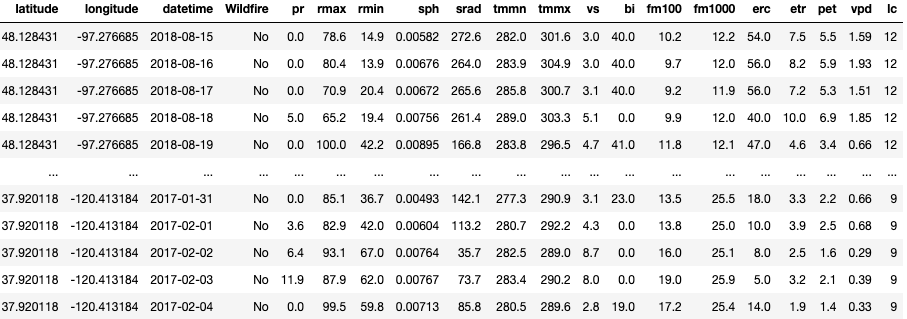
\includegraphics[width=1\linewidth]{images/dataset_snapshot.png}
    \caption{Snapshot of the 9.5 million-record meteorological dataset showing the 15-feature temporal structure across the 75-day observation window.}
\label{fig:dataset_snapshot}
\end{figure}

This high-resolution, multi-modal dataset forms the foundation for wildfire ignition prediction and realistic scenario simulation in subsequent pipeline stages.

\subsection{Stage 2: Wildfire Ignition Forecasting}

We designed a deep learning model to forecast wildfire ignition based on the 75-day meteorological and environmental context window described in Stage 1. The model treats the task as a binary classification problem: given a sequence of atmospheric and fire-related covariates, predict whether a fire will ignite at the target (coordinate, timestamp) location.

The wildfire predictor is a hybrid CNN-LSTM-Attention architecture that captures both spatial correlations and temporal dynamics. A detailed architecture is shown in Figure~\ref{fig:cnn_lstm_model}

\begin{figure}[htbp]
    \centerline{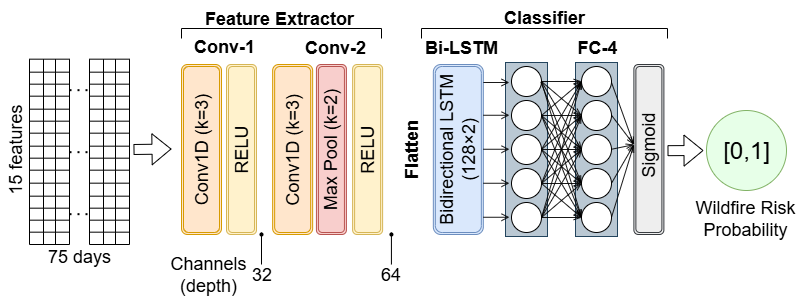
\includegraphics[width=1\linewidth]{images/dl_nn.png}}
    \caption{The architecture of the Neural Network model used for wildfire prediction}
    \label{fig:cnn_lstm_model}
\end{figure}


% \noindent
% \textbf{Model.} A hybrid CNN–LSTM network encodes local spatial structure and long-range temporal dynamics, respectively. Trained with focal loss and class-balanced sampling, the model attains \textbf{73.1\% accuracy} on a held-out years (2023-25).

% \noindent
% \textbf{Deployment.} A lightweight web front-end allows users to select a location and date; the back-end automatically assembles the corresponding 75-step feature window and returns a fire-ignition probability. The system correctly flagged the \textsc{California} wildfire of \textsc{7 Jan 2025} a day in advance.

\subsection{Stage 3: RL-Based Helitack Suppression}

Once the predicted wildfire ignition probability exceeds 50\%, we construct a 3D terrain model and launch a physics-aware fire-spread simulation that streams live elevation, land-cover, and mesoscale wind fields. Although the engine omits several meteorological predictors (e.g.\ solar radiation, long-term humidity), it provides a sufficiently realistic sandbox for tactic optimization.

\subsubsection{Custom Reinforcement Learning Environment}

The simulation environment is built upon a Cellular Automata (CA) engine, embedded in a custom Gymnasium wrapper. This design provides a step-wise fire progression and real-time agent interaction within a spatially grounded 3D simulation.


% \textbf{Web-to-Gym bridge.} The Three.js client connects via WebSockets to a custom \texttt{gymnasium} environment hosting the fire engine; the blaze is ignited at the predicted coordinates, and slope-wind-fuel interactions drive its spread.

% \noindent
% \textbf{Helitack agent.} A Stable Baselines 3 PPO agent~\cite{stable-baselines} built on a four-frame CNN encoder, LSTM context, and Slot-Attention—learns water-drop locations, sortie timing, and evacuation triggers. A reward balances burned-area reduction, drop cost, and loiter penalties. After $3{\times}10^{5}$ training steps, the agent reliably "circles" the flame front and slows growth in held-out terrains.

% \noindent
% \textbf{Logged outputs.} During each roll-out we record helitack coordinates, burned-area trajectory, and ignition metadata; these feed Stage 3's \emph{Fire Threat Assessment Report}.


% \subsubsection{Model Building}

% The predictor model is a classifier that predicts wildfire or no-wildfire label based on the 75 day data window. The model is a deep neural network model (see image) with multiple LSTM and CNN layers, along with attention layers. The data set was divided into train,validation and test sets in 7:2:1. The model was also trained on CCR \cite{ccr}. The model managed to achieve an accuracy of \textbf{73.1}\% on the test set. Notably the model predicted the Palisades Wildfires of California on January 2025 with \textbf{98.6}\% confidence.


% \subsection{Mitigation of Wildfires \& Reinforcement Learning Framework}

% \subsubsection{The Environment}
% The environment is a Cellular Automata inspired dynamic wildfire simulation environment embedded in a custom Gymnasium wrapper, allowing the RL agent to learn fire suppression methodologies within a physics based system.

% \paragraph{Code Foundation}

% We adapted the simulation backend from the Concord Consortium's Wildfire Model~\cite{concord_consortium}. The visual rendering is implemented in Three.js and React, representing a 240\(\times\)160 cell terrain slice, with elevation layers derived from real-world DEM data.

% \paragraph{Cellular Automata Dynamics}
% Each cell stores spatial and fire-related state:
% \begin{itemize}
%     \item \texttt{x}, \texttt{y}: grid coordinates
%     \item \texttt{zone}: vegetation and terrain fuel properties
%     \item \texttt{baseElevation}, \texttt{spreadRate}, \texttt{burnTime}, \texttt{fireState}
%     \item \texttt{helitackDropCount}, \texttt{isFireSurvivor}, \texttt{ignitionTime}
% \end{itemize}
% State transitions follow discrete-time updates based on fuel, slope, and wind conditions.




% The environment is a Cellular Automata inspired dynamic wildfire simulation environment which has a 2D grid of cells where each cell has a state. Each cell state has following attributes -

% \begin{enumerate}
%     \item \texttt{x}, \texttt{y}: Integer coordinates representing the cell's location in the 2D simulation grid.
    
%     \item \texttt{zone}: A \texttt{Zone} object containing vegetation and terrain properties associated with the cell like fuel values.
    
%     \item \texttt{baseElevation}: Elevation of the cell (in meters), used for slope-based fire spread calculations.
    
%     \item \texttt{ignitionTime}: Time step (or simulation time) at which the cell caught fire; initialized to \texttt{inf} for unignited cells.
    
%     \item \texttt{spreadRate}: Dynamic rate of fire spread (e.g., in m/s) from this cell, computed using the Rothermel model.
    
%     \item \texttt{burnTime}: Remaining time the cell will continue burning after ignition, initialized to \texttt{MAX\_BURN\_TIME}.
    
%     \item \texttt{fireState}: Enum representing the current fire state of the cell (\texttt{Unburnt}, \texttt{Burning}, or \texttt{Burnt}).
    
%     \item \texttt{helitackDropCount}: Integer tracking how many times suppressant has been dropped on this cell by helitack units.
    
%     \item \texttt{isFireSurvivor}: Boolean flag denoting whether the cell survived fire due to intervention or natural factors.
% \end{enumerate}

% Your simulation evolves over discrete time steps, and state transitions happen stepwise.\\
% The fire spreads to neighboring cells based on a fire engine that computes the spread of fire.

% \paragraph{Fire Engine and Fuel Constants}
% The fire engine in the environment is a core simulation module that computes the fire ignition, spread rate of the ongoing fire and extinguishing dynamics.\\
% The fire engine based on \textbf{Rothermel's fire spread equation} \cite{rothermel_fire_spread_eq}, simplified for a 2D grid following standard fire simulators like \textbf{FARSITE} \cite{finney2004farsite}.\\
% The fire engine calculates the rate of fire spread from a burning cell to neighboring cells based on Rothermel's fire spread equation that uses land cover/vegetation-dependent parameters.

% \paragraph{Fuel Parameters Used}
% \begin{enumerate}
%     \item \texttt{SAV:} Surface Area-to-Volume Ratio
%     \item \texttt{Net Fuel Load:} Dry fuel available
%     \item \texttt{Fuel Bed Depth:} Fuel height/depth
%     \item \texttt{Packing Ratio:} Fuel compactness
%     \item \texttt{Moisture Of Extinction (mx):} Moisture threshold for combustion
% \end{enumerate}

% \paragraph{Source of Fuel Parameters}
% The simulation uses fuel parameters for different land covers loosely derived and adapted from Anderson’s 13 Fuel Models and Scott \& Burgan’s 40 Fuel Models normalized for simulation and tuned for stability and realism.

% \paragraph{Fire Spread Calculations}
% Each cell tracks the \texttt{Ignition Time} and \texttt{Time Remaining for Burning}. The fire spread is calculated based on above mentioned cell properties and the influence of other factors such as wind speed, local elevations and flammability of vegetation of neighboring cells.\\

% Rothermel’s 1972 model calculates the rate of fire spread $R$ in surface fuels using:

% \begin{equation}
% R = \frac{I_R \cdot \xi}{\rho_b \cdot \epsilon \cdot Q_{ig}}
% \end{equation}

% where:
% \begin{itemize}
%     \item \( R \) is the forward rate of spread (m/s),
%     \item \( I_R \) is the reaction intensity (kW/m\(^2\)),
%     \item \( \xi \) is the propagating flux ratio (dimensionless),
%     \item \( \rho_b \) is the oven-dry bulk density (kg/m\(^3\)),
%     \item \( \epsilon \) is the effective heating number (dimensionless),
%     \item \( Q_{ig} \) is the heat of pre-ignition (kJ/kg).
% \end{itemize}

% The final spread rate including wind and elevation effects is:

% \begin{equation}
% R_{\text{eff}} = R \cdot \left(1 + \Phi_w + \Phi_s\right)
% \end{equation}

% where:
% \begin{itemize}
%     \item \( \Phi_w \) is the wind factor,
%     \item \( \Phi_s \) is the elevation factor.
% \end{itemize}

% The wind factor \( \Phi_w \) and elevation factor \( \Phi_s \) are calculated as:

% \begin{equation}
% \Phi_w = C \cdot U^B \cdot \left( \frac{\beta}{\beta_{\text{opt}}} \right)^{-E}
% \end{equation}

% \begin{equation}
% \Phi_s = 5.275 \cdot \beta^{-0.3} \cdot \tan^2 \theta
% \end{equation}

% where:
% \begin{itemize}
%     \item \( U \) is the mid-flame wind speed (ft/min),
%     \item \( \beta \) is the packing ratio,
%     \item \( \beta_{\text{opt}} \) is the optimum packing ratio,
%     \item \( \theta \) is the elevation angle,
%     \item \( C, B, E \) are fuel-specific empirical coefficients.
% \end{itemize}
% There is a factor added for adding some stochasticity to emulate the fire dying out by itself or due to natural reasons.

% \paragraph{Customizing the Environment}
% The boilerplate code was modified to create a highly realistic render for which we used satellite-based datasets MODIS(Moderate Resolution Imaging Spectroradiometer) and SRTM (Shuttle Radar Topography Mission) via the Google Earth Engine SDK\cite{earth_engine}. We extracted the land cover maps from MODIS, elevations from SRTM and wind speed data from GridMET \cite{gridmet}.

% The land cover is of the following types:

% \begin{enumerate}
%     \item Evergreen Needleleaf Forests
%     \item Evergreen Broadleaf Forests
%     \item Deciduous Needleleaf Forests
%     \item Deciduous Broadleaf Forests
%     \item Mixed Forests
%     \item Closed Shrublands
%     \item Open Shrublands
%     \item Woody Savannas
%     \item Savannas
%     \item Grasslands
%     \item Permanent Wetlands
%     \item Croplands
%     \item Urban and Built-Up Lands
%     \item Cropland/Natural Vegetation Mosaics
%     \item Snow and Ice
%     \item Barren or Sparsely Vegetated
%     \item Water Bodies
% \end{enumerate}

% The land cover and elevations are downloaded as GeoTIFF images and converted to numpy arrays.\\ 
% These properties are then mapped to the cells and fed to Three.js to render the environment.

% \begin{figure}[!h]
%     \centering
%     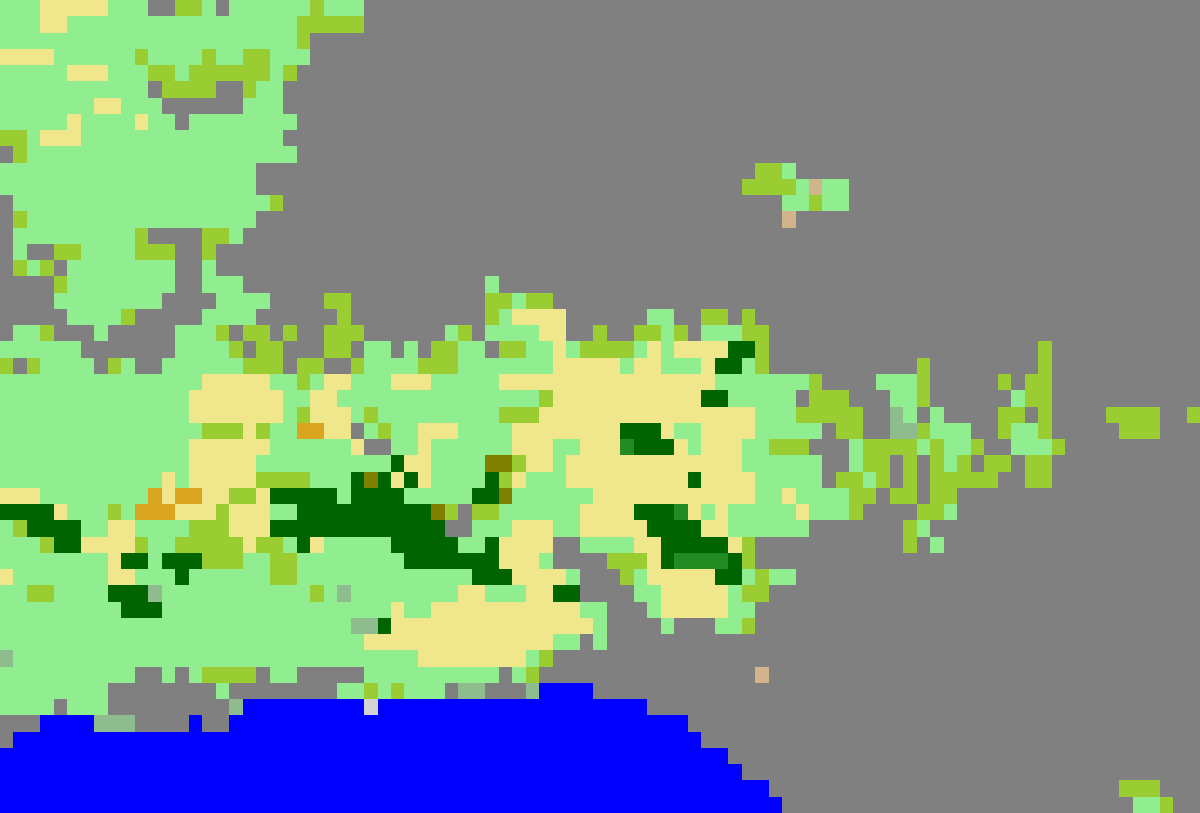
\includegraphics[width=0.75\linewidth]{images/landcover_1.png}
%     \caption{Land cover map from MODIS via Google Earth Engine}
% \end{figure}

% \begin{figure}[!h]
%     \centering
%     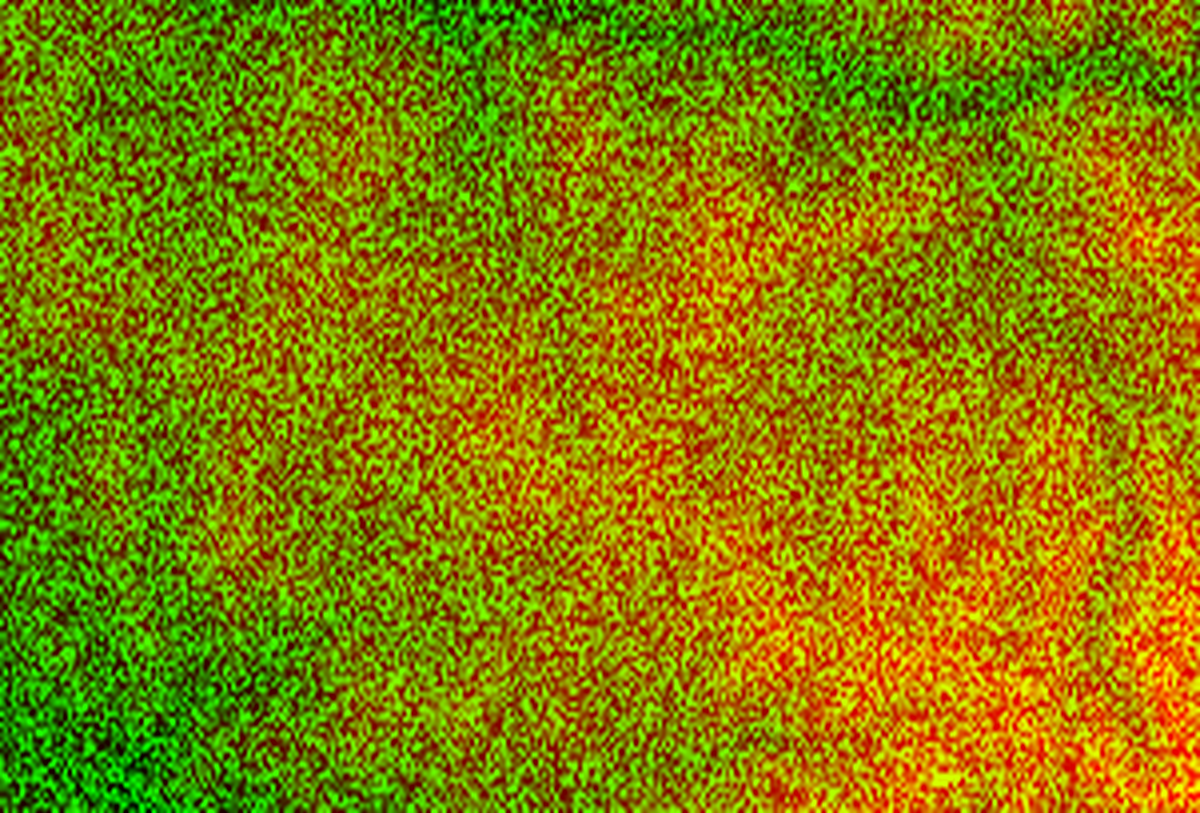
\includegraphics[width=0.75\linewidth]{images/heightmap_1.png}
%     \caption{Height Map from SRTM via Google Earth Engine}
% \end{figure}
% \subsubsection{Engineering a custom Gymnasium environment}
% To train a Reinforcement Learning agent on this simulation environment, we needed a python-based custom gymnasium environment connected to the browser-based fire engine. We used python websockets and asyncio for the state and action updates between gymnasium and the Cellular Automata cell state. \\
% This allowed us to decouple the visualization from the python based visualization libraries to a more realistic Javascript based 3D render in the browser.\\

% \begin{figure}[!h]
%     \centering
%     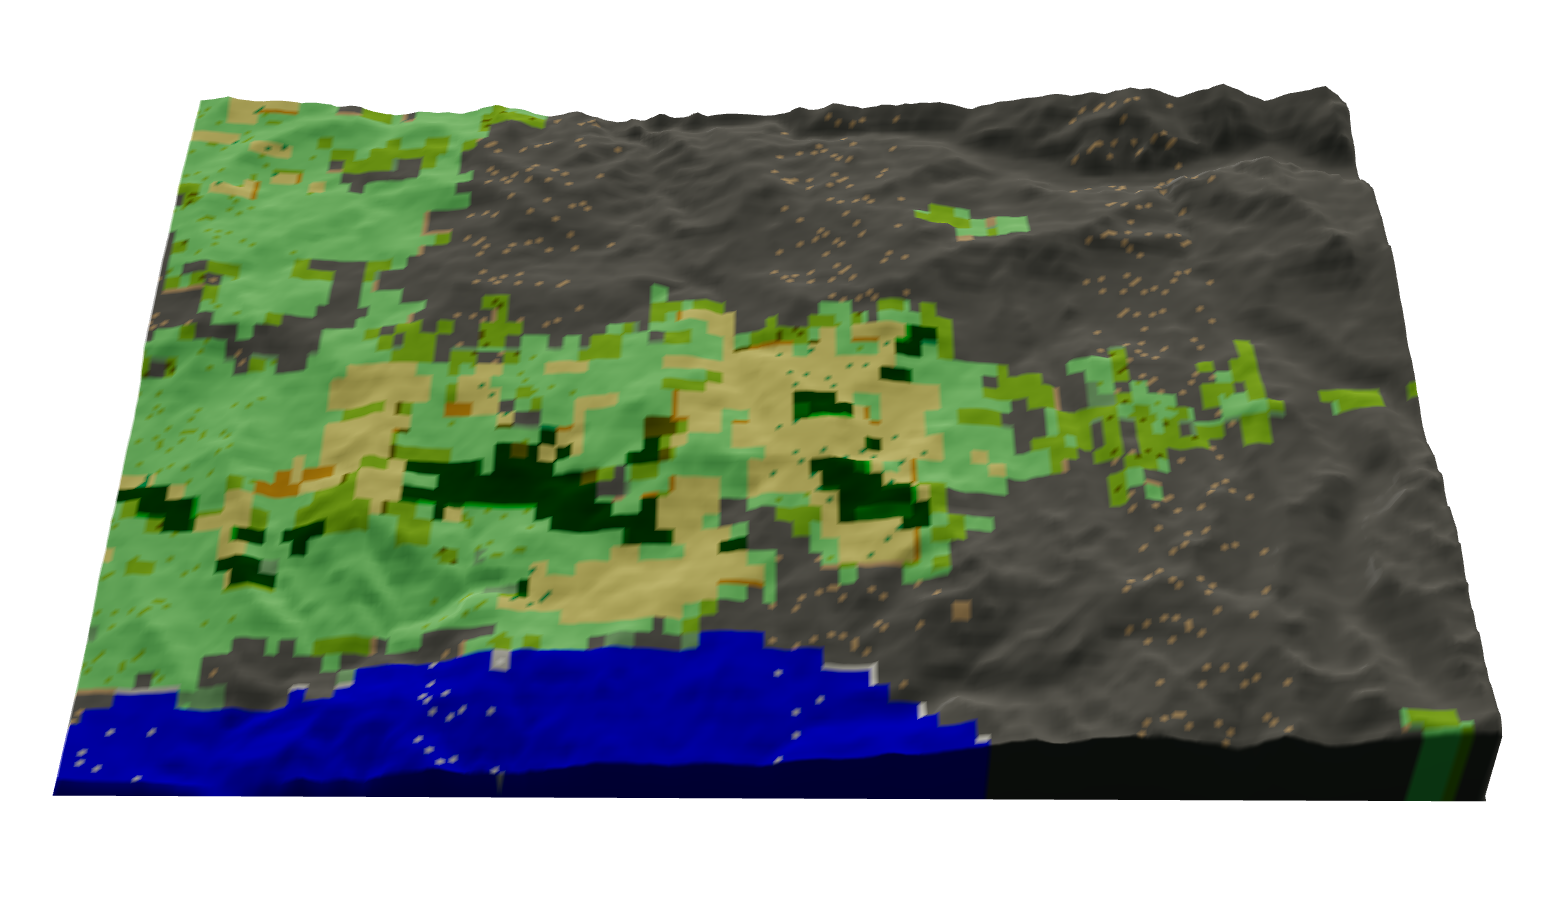
\includegraphics[width=0.75\linewidth]{images/environment_render.png}
%     \caption{The environment rendered in the browser}
% \end{figure}

% \subsubsection{The Agent and Reinforcement Learning}
% The agent is a helitack chopper - it is an aerial firefighting unit that can move and drop fire suppressant/water on burning cells known as Helitack.

% \paragraph{Action Space}
% The Helitack agent has the following action space:
% \begin{enumerate}
%     \item Navigate Up
%     \item Navigate Down
%     \item Navigate Left
%     \item Navigate Right
%     \item Drop water/suppressant
% \end{enumerate}

% \paragraph{Observation Space}
% The observation space has the following:
% \begin{itemize}
%     \item \texttt{Binned Cells:} 2D matrix of cells discretized into 8 bins based on the state of the cell (Unburnt (0), Burning(1) and Burnt(2) and intensity of fire(Low(0), Medium(1) and High(2)). 
%     \begin{equation}
%     FireState * 3 + BurnIndex
%     \end{equation}
%     It is set to -1 if the cell's vegetation is nonburnable.
%     \item \texttt{Agent Coordinates:} Coordinates of the helitack agent
%     \item \texttt{Agent On Fire:} A boolean variable denoting weather the agent is on a burning cell.
% \end{itemize}

% \paragraph{The Reward Function}
% From the observation space, we can extract a lot of useful metrics per step to formulate an efficient reward function:
% \begin{itemize}
%     \item Currently burning cell count
%     \item Extinguished by the agent cell count
%     \item Burnt cell count
%     \item Previously Burnt cell count
%     \item Newly Burnt cell count
% \end{itemize}
% The reward function for the Helitack agent should have the following salient features:
% \begin{enumerate}
%     \item Encourage containment/suppression - Positive reward for suppressing fire or containing it.
%     \item Positive rewards for preempting fire growth
%     \item Negative reward for burned area
%     \item Penalty for flying over burned or nonburnable zones
% \end{enumerate}


\paragraph{Code Foundation}
Our simulation backend is adapted from the Concord Consortium's Wildfire Model~\cite{concord_consortium}. A React and Three.js-based frontend renders the terrain as a 240\(\times\)160 grid, layered with digital elevation maps (DEM) and real-time vegetation data. The simulation logic and RL integration run on Python, with the frontend and backend linked via WebSockets using \texttt{asyncio}.

\paragraph{Cell Structure and State Variables}
Each cell in the grid is modeled as a discrete CA unit with the following attributes:
\begin{itemize}
    \item \texttt{x}, \texttt{y}: grid coordinates
    \item \texttt{zone}: terrain and vegetation type with fuel properties
    \item \texttt{baseElevation}: ground elevation (m)
    \item \texttt{spreadRate}: local fire spread velocity (m/s)
    \item \texttt{burnTime}: time remaining until burnout
    \item \texttt{fireState}: one of \texttt{Unburnt}, \texttt{Burning}, or \texttt{Burnt}
    \item \texttt{ignitionTime}: simulation timestamp of ignition
    \item \texttt{helitackDropCount}: suppressant drop count
    \item \texttt{isFireSurvivor}: boolean flag for fire escape
\end{itemize}
Simulation state transitions evolve over discrete time steps, incorporating terrain slope, wind direction, and vegetation characteristics.

\paragraph{Fire Engine and Spread Modeling}
At the core is a fire engine module based on Rothermel’s fire spread equation~\cite{rothermel_fire_spread_eq}, adapted for grid-based simulators such as \textbf{FARSITE}~\cite{finney2004farsite}. The rate of spread $R$ is computed as:
\begin{equation}
R = \frac{I_R \cdot \xi}{\rho_b \cdot \epsilon \cdot Q_{ig}}
\end{equation}
where $I_R$ is reaction intensity, $\xi$ is the propagating flux ratio, $\rho_b$ is bulk density, $\epsilon$ is the heating number, and $Q_{ig}$ is the ignition heat.

Environmental effects are captured via:
\begin{equation}
R_{\text{eff}} = R \cdot (1 + \Phi_w + \Phi_s)
\end{equation}
where $\Phi_w$ and $\Phi_s$ represent wind and slope adjustments, respectively.

\paragraph{Fuel Models and Parameters}
Each vegetation type includes the following properties:
\begin{itemize}
    \item \texttt{SAV}: Surface area-to-volume ratio
    \item \texttt{Net Fuel Load}: Dry fuel available
    \item \texttt{Fuel Bed Depth}: Vertical extent of combustibles
    \item \texttt{Packing Ratio}: Fuel density
    \item \texttt{Moisture of Extinction (mx)}: Minimum moisture for combustion
\end{itemize}
These values are derived from Anderson’s 13 Fuel Models and Scott \& Burgan’s 40 Fuel Models and normalized for simulation.

\paragraph{Realistic Terrain and Vegetation Integration}
To achieve realism, we integrate satellite-derived data via Google Earth Engine~\cite{earth_engine}:
\begin{itemize}
    \item Land cover from MODIS
    \item Elevation data from SRTM
    \item Wind field estimates from GridMET~\cite{gridmet}
\end{itemize}
Land covers include forests, shrublands, grasslands, croplands, wetlands, urban areas, and more. These are stored as GeoTIFFs and converted to NumPy arrays for spatial mapping.

% \begin{figure}[!h]
%     \centering
%     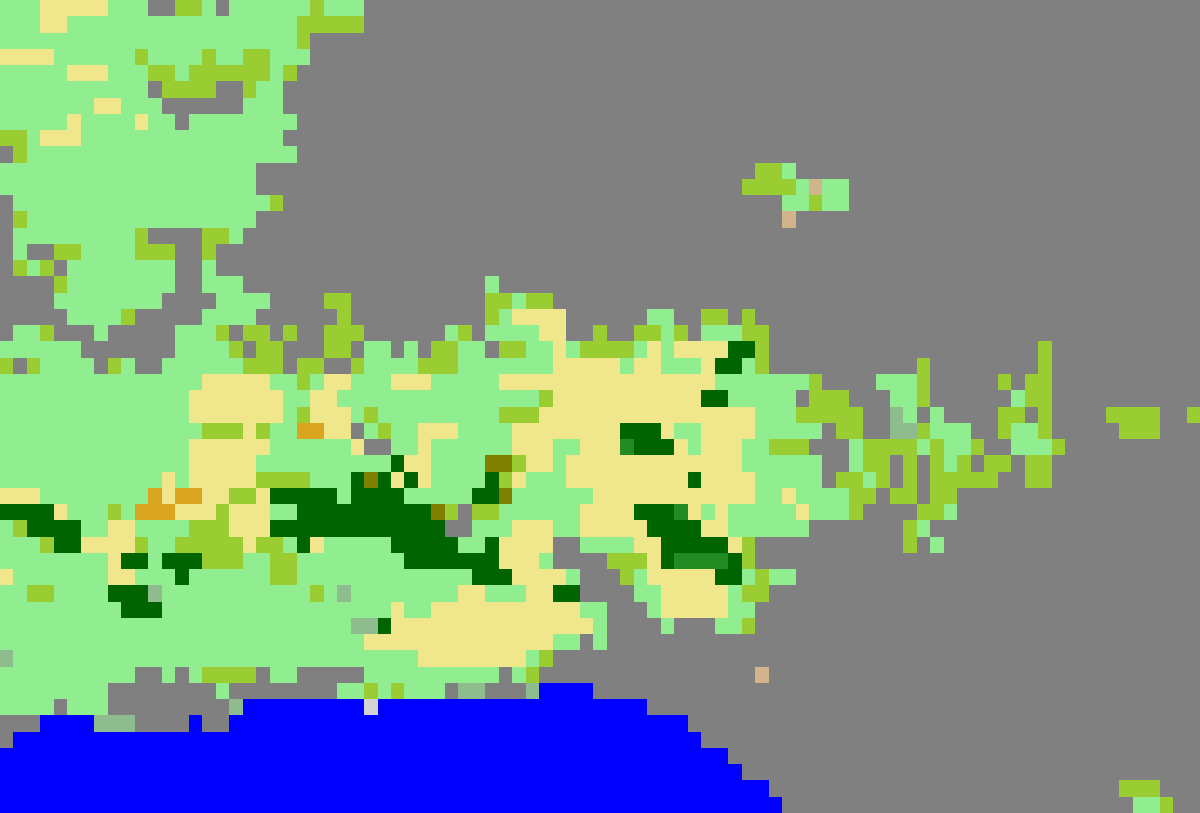
\includegraphics[width=0.75\linewidth]{images/landcover_1.png}
%     \caption{Land cover map from MODIS via Google Earth Engine}
% \end{figure}

% \begin{figure}[!h]
%     \centering
%     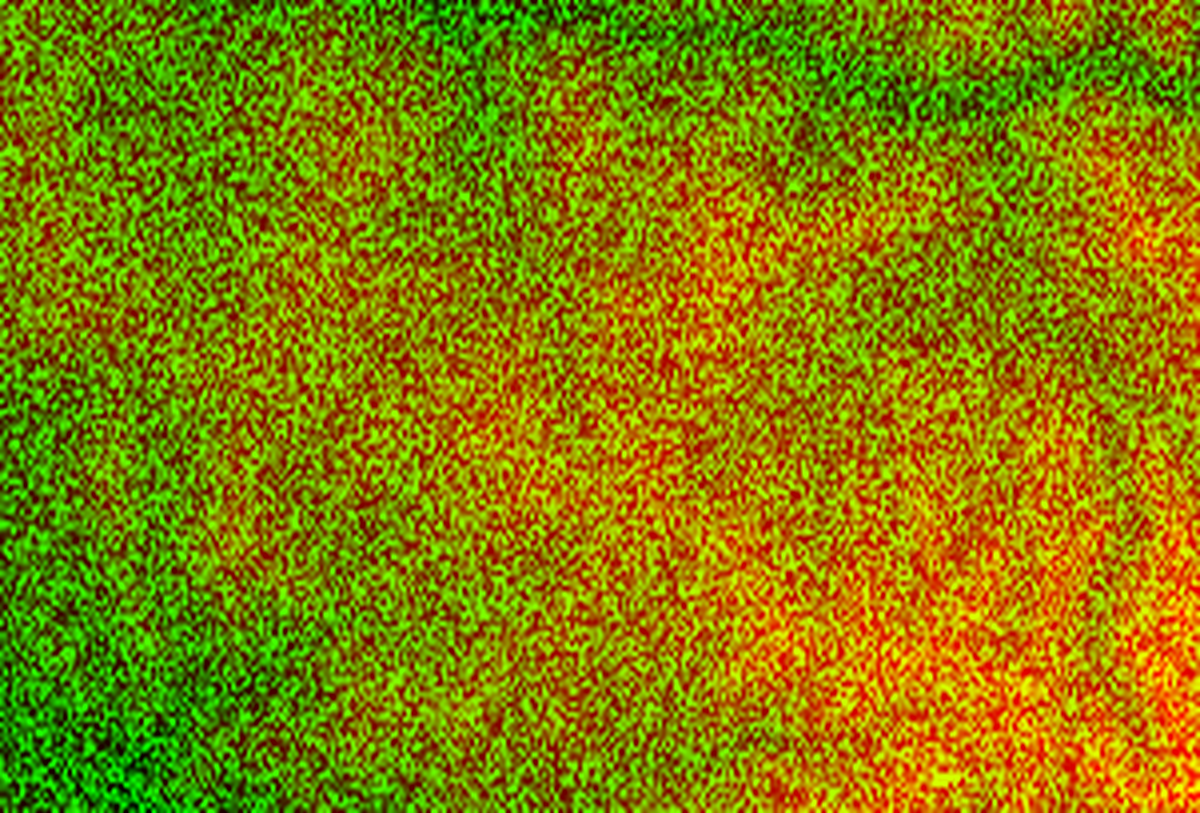
\includegraphics[width=0.75\linewidth]{images/heightmap_1.png}
%     \caption{Height Map from SRTM via Google Earth Engine}
% \end{figure}

\paragraph{Gymnasium Integration and WebSocket Bridge}
The Gymnasium wrapper supports the simulation as an RL environment with step/reset APIs. Python-based WebSocket and \texttt{asyncio} interfaces provide bidirectional communication with the browser-based fire engine. This design provides us with both rendering and computation, allowing RL agents to train while visualizations run in React/Three.js.

% \begin{figure}[!h]
%     \centering
%     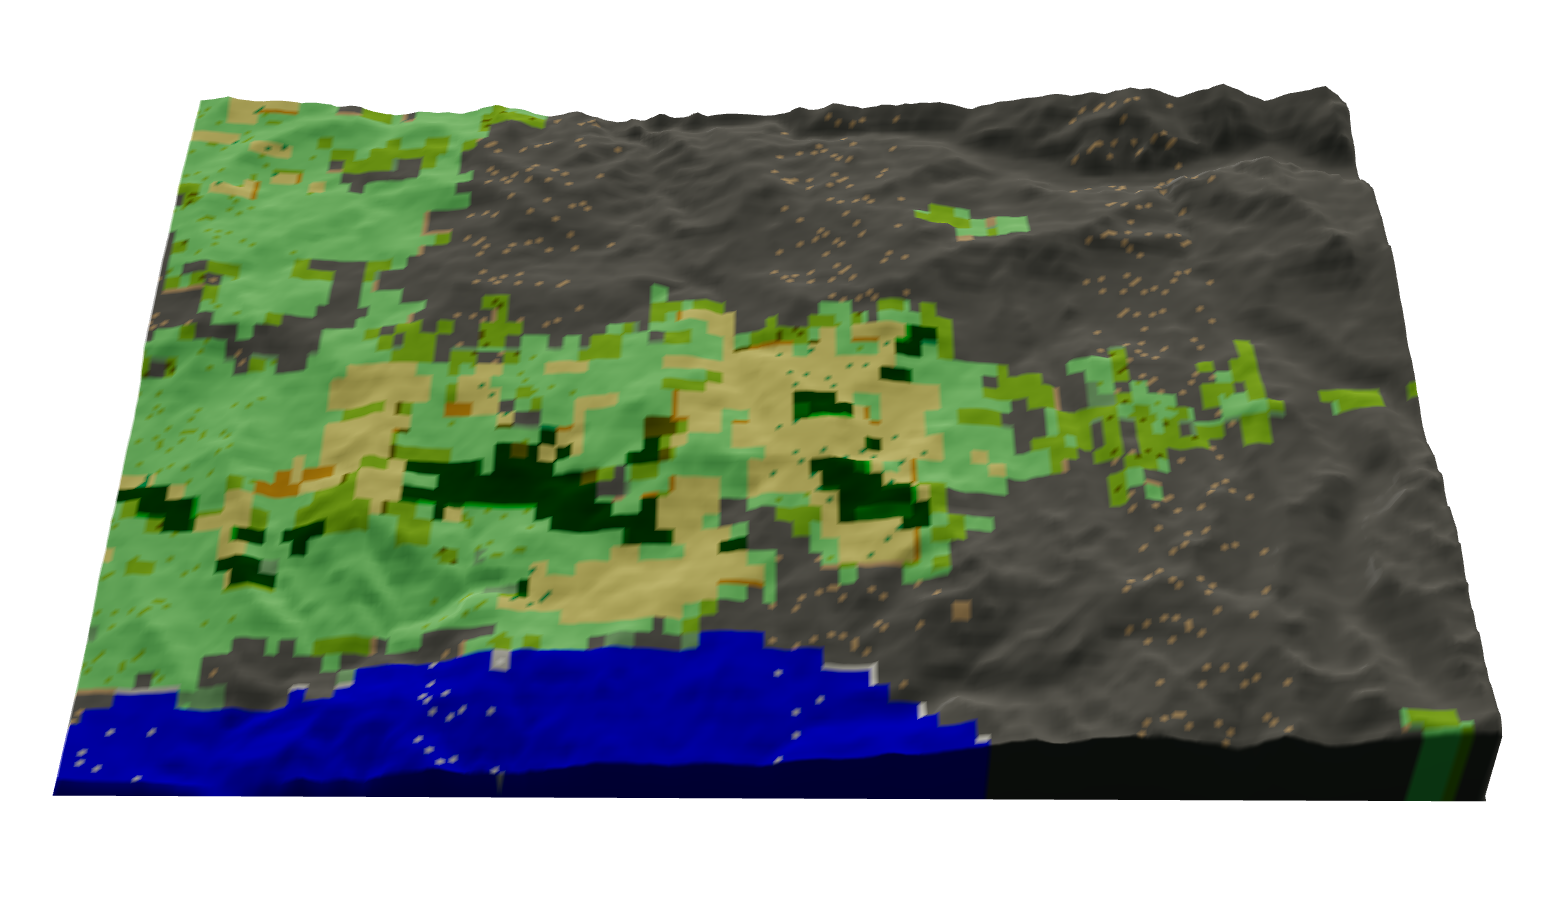
\includegraphics[width=0.75\linewidth]{images/environment_render.png}
%     \caption{The environment rendered in the browser}
% \end{figure}

\begin{table*}[htbp]
\centering
% \resizebox{\textwidth}{!}{%
\begin{tabular}{|c|c|c|c|}
\hline
\textbf{Earth Engine} & \textbf{Landcover} & \textbf{Heightmap} & \textbf{Final 3D Render} \\
\hline
\centering
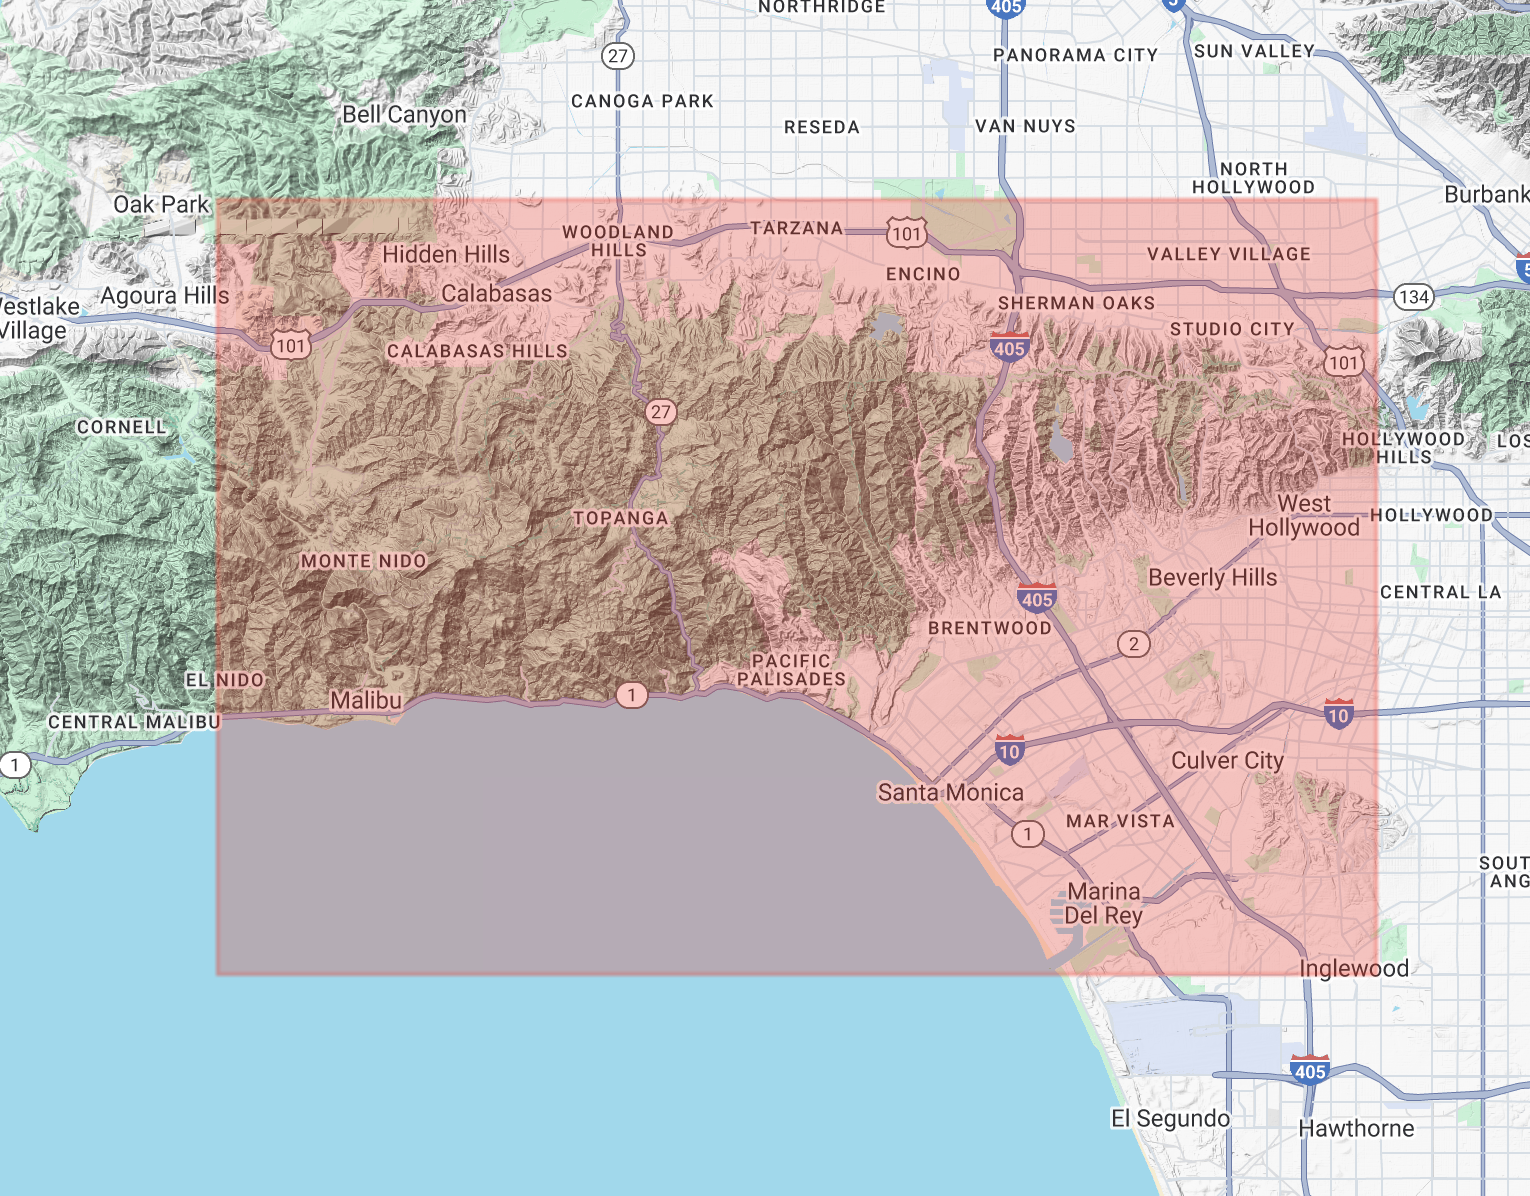
\includegraphics[width=0.22\textwidth]{images/earth_engine_env1.png} & 
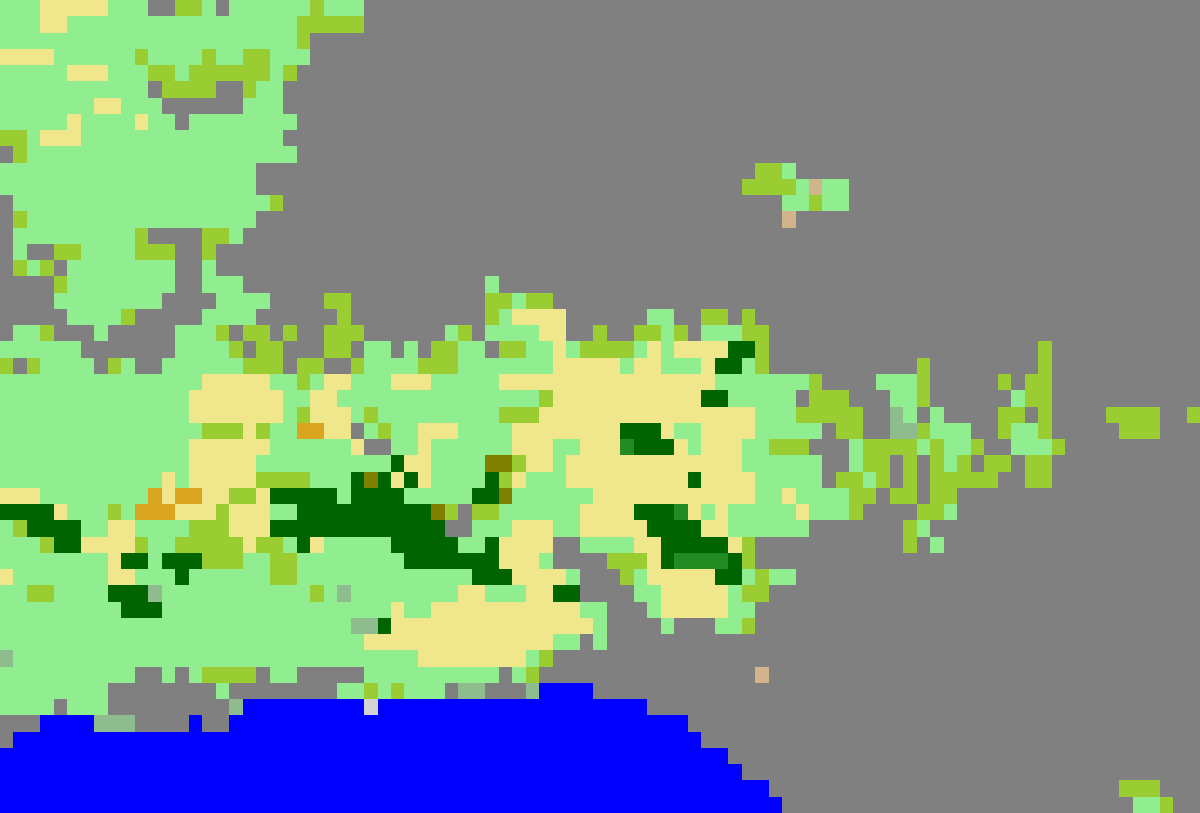
\includegraphics[width=0.22\textwidth]{images/landcover_1.png} & 
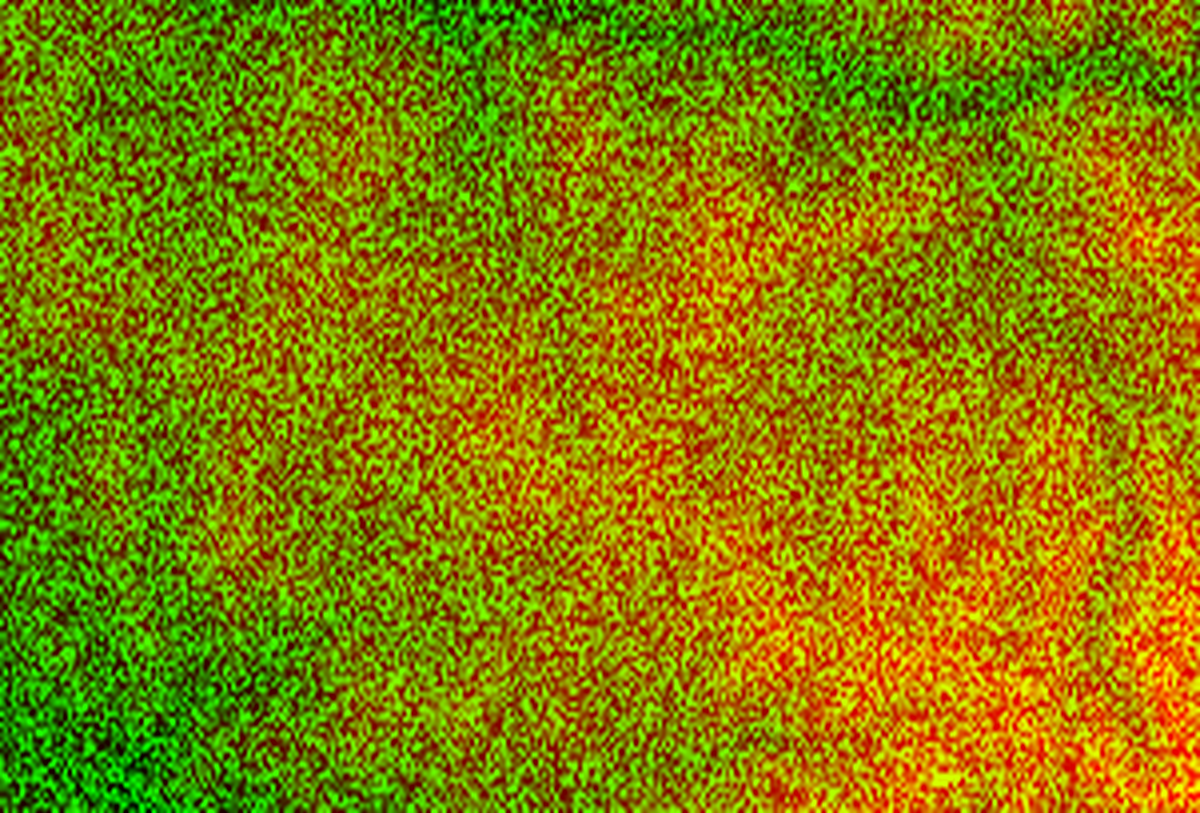
\includegraphics[width=0.22\textwidth]{images/heightmap_1.png} & 
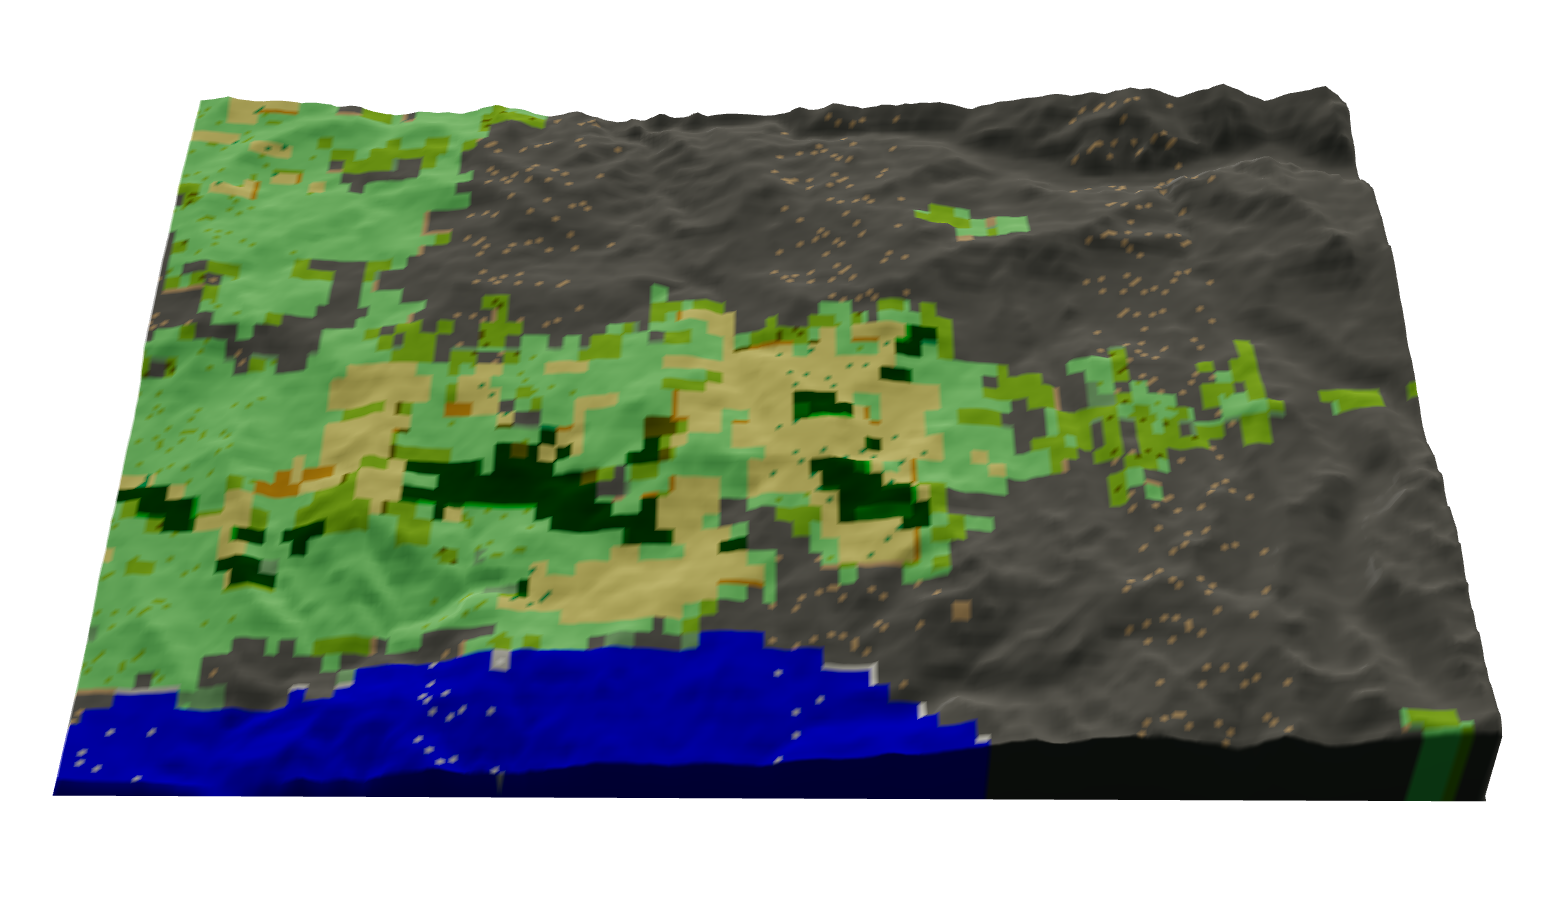
\includegraphics[width=0.25\textwidth]{images/environment_render.png} \\
\hline
\end{tabular}%
% }
\caption{
Four stages of environment creation for simulation: (1) region selection using Google Earth Engine, (2) extracted land cover raster (GeoTIFF), (3) corresponding elevation map (heightmap TIFF), and (4) the final rendered simulation environment with terrain and vegetation.
}
\label{tab:wildfire_environment_creation}
\end{table*}


\paragraph{Proximal Policy Optimization (PPO)}
We adopt the Proximal Policy Optimization (PPO) \cite{schulman2017ppo} as the core reinforcement learning algorithm for training our helitack agent. PPO is a clipped policy gradient method known for its stability, robustness, and sample efficiency in complex environments with high-dimensional observations. 

% It strikes a balance between:
% \begin{itemize}
%     \item Robust learning (via clipped objective function to avoid large destructive updates)
%     \item On-policy training (ideal for environments with changing dynamics)
%     \item Compatibility with neural network architectures.
% \end{itemize}

PPO is particularly well-suited for our wildfire suppression scenario due to:
\begin{itemize}
    \item State transitions are non-stationary (fire behavior changes with suppression, terrain, and fuel)
    \item The agent's effect is localized and sequential (dropping suppressant affects the future spread)
    \item Exploration is challenging due to sparse rewards.
\end{itemize}

We build on Stable-Baselines3’s \cite{stable-baselines3} PPO implementation, modifying the policy network to accommodate spatiotemporal features relevant to fire dynamics.

\paragraph{Action Space}
\begin{itemize}
    \item Discrete moves: Up, Down, Left, Right
    \item Drop suppressant (binary)
\end{itemize}

\paragraph{Observation Space}
The agent receives the following observations:

\begin{itemize}
    \item \texttt{cells}: A 4-frame stack of 160\(\times\)240 environment grids capturing fire states (unburnt, burning, burnt) and intensities over time;
    \item \texttt{helicopter\_coord}: Current agent position in the simulation grid;
    \item \texttt{on\_fire}: Binary flag indicating whether the agent is positioned over a burning cell.
\end{itemize}

\paragraph{Reward Function}
The reward function is based on short-term suppression with long-term containment by considering both state-based and proximity-aware feedback:
\begin{itemize}
    \item Positive rewards: 
        \begin{itemize}
            \item for extinguishing burning cells,
            \item for preventing fire expansion by timely drops,
            \item for maintaining proximity to fire fronts.
        \end{itemize}
    \item Negative penalties:
        \begin{itemize}
            \item for fire growth or large burned area,
            \item for inaction or delayed intervention,
            \item for hovering over burnt or inert terrain.
        \end{itemize}
\end{itemize}
This reward function encourages the intelligent suppression strategies such as dynamic circling of fire fronts, firebreak creation, and early response to high-risk areas.

\paragraph{Feature Extractor Design: CNN + LSTM + Attention}
To encode this structured observation, we design a custom feature extractor combining:
\begin{enumerate}
    \item Multi-Scale Convolutional Neural Network (CNN)
    We use three parallel CNN branches to capture patterns at multiple scales:
    \begin{itemize}
        \item Small receptive field (3×3): captures local flame structure.
        \item Medium receptive field (5×5): captures fire clusters and propagation zones.
        \item Large receptive field (11×11): captures global fire spread patterns.
    \end{itemize}
    Each CNN output is interpolated to a common spatial shape and concatenated into a single feature map.
    \item Spatial Attention Mechanism
    To guide the network’s focus on critical fire zones, we apply a spatial attention module:

    \[
    \text{AttendedMap} = \sigma\left( \text{Conv}_{1 \times 1} \left( \text{ReLU} \left( \text{Conv}_{1 \times 1}(F) \right) \right) \right)
    \]
    The attention map is multiplied element-wise with the multi-scale CNN output, encouraging the model to emphasize informative spatial regions.

    \item LSTM for Temporal Encoding
    The flattened spatial features are passed through a two-layer LSTM, allowing the agent to learn from historical dynamics of fire behavior and past actions.

    The LSTM captures:
    \begin{itemize}
        \item Temporal consistency of fire growth
        \item Lagged effects of suppression actions
        \item Dynamic state transitions in the environment.
    \end{itemize}
\end{enumerate}

\paragraph{Merging Other inputs}
Alongside visual features, we process:
\begin{itemize}
    \item Helitack coordinates (absolute and relative): passed through a coordinate encoder (2-layer MLP).
    \item on\_fire flags: passed through a shallow MLP to indicate fire-contact state.
\end{itemize}
All extracted features are concatenated into a fused representation, followed by a 2-layer fully connected residual block to produce the final policy and value features.

A detailed architecture is presented on Fig.~\ref{fig:ppo_flowchart}

% \paragraph{Training Setup}

\begin{figure*}[htbp]
\centerline{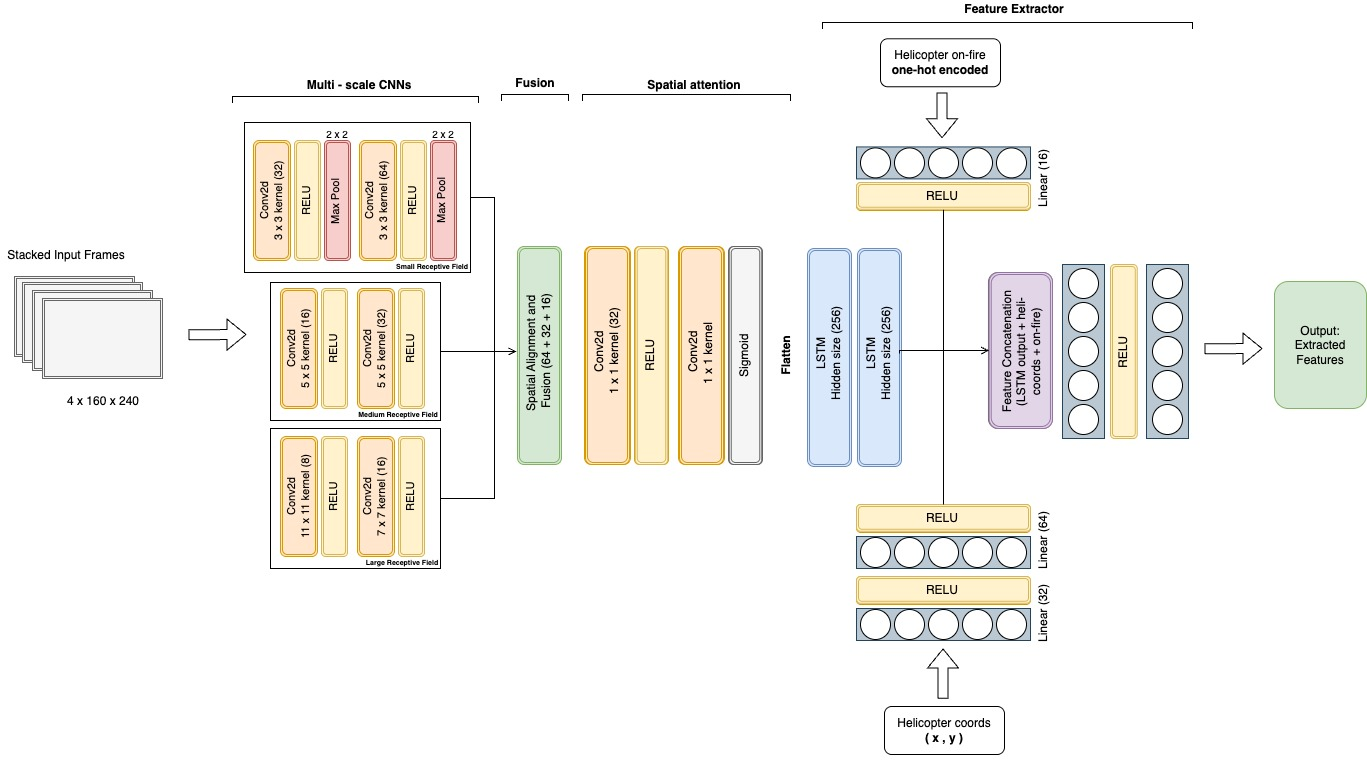
\includegraphics[width=1\linewidth]{images/RL_NN.jpg}}
\caption{Custom PPO Policy architecture}
\label{fig:ppo_flowchart}
\end{figure*}

% \subsubsection{The reward function}

% The reward function is carefully designed to promote effective wildfire suppression strategies. It positively reinforces direct fire extinguishment actions and encourages proximity to actively burning areas through a proximity-based exponential reward. Simultaneously, it penalizes the expansion of fire, ongoing burning, and time spent without meaningful intervention. Strategic behaviors, such as deploying helitack near burning regions to create firebreaks, are rewarded, while misdirected actions—such as deploying resources on already burnt or unaffected areas—incur penalties. This design ensures the agent learns to balance immediate suppression with longer-term containment strategies, closely mimicking real-world decision-making in wildfire response.



\subsection{Stage 4: Fire Threat Assessment Report \& Helitack Strategy}

During each validation rollout, we log:
\begin{itemize}
    \item Helitack deployment log: Coordinates and timestamps of each suppressant drop, organized by sortie sequence.
    \item Burned area trajectory
    \item Predicted ignition coordinates, time of ignition, and confidence score from the forecasting stage.
    \item Total number of helitack deployments, total fireline length impacted, time elapsed before containment.
    \item Suggested evacuation advisories, suppression prioritization zones, and contingency thresholds.
\end{itemize}

% During the simulation, we track all metrics:
% Total count of helitacks used, Total Burnt area, Coordinates to drop helitacks by the agent, Total Time Elapsed.

We use all these metrics to prepare a PDF report "Fire Threat Assessment Report". The report offers decision-makers a real-time operational summary, integrating forecasted ignition patterns with the simulated suppression plan. 

% , to help the reader infer the severity of the predicted fire and use the relevant metrics to be prepared in case the wildfire disaster takes place.

% During each validation roll-out we log:

% \textbf{Helitack drop coordinates \& sortie sequence}, \textbf{Burned area trajectory}: Burnt acreage over simulation time, \textbf{Ignition metadata}: forecasted ignition time and coordinates, and \textbf{Action plan}: evacuation advisories, resource allocations, contingency triggers.

% These elements are auto-compiled into a single-page \emph{Fire Threat Assessment Report} delivered within minutes of a high-risk forecast.

\subsection{Stage 5: Web Interface}
We developed a web-based application using Flask and React for users to predict wildfire probability at a location/coordinate. The Inferno UI uses Leaflet which is a navigable map with location picker and calls the backend with the coordinates and date time to make a prediction. The backend uses these coordinates and date time and the calls the GRIDMET API and GRIDMET forecast API to prepare the 75 day window with weather data for the trained model to make a prediction.

If the wildfire prediction model predicts a confidence greater than 50\%, we navigate to Tactics (simulation page). The backend then uses the Google Earth Engine python SDK to create the exact cross section of the predicted wildfire using the elevation and land cover data. The trained agent simulates over this rendered environment and tracks the relevant metrics as mentioned in section 4.2 to prepare the Threat assessment report.


\section{Results}

We evaluate the performance of our proposed pipeline across three core stages: (i) data acquisition, (ii) wildfire-ignition forecasting using spatio-temporal deep learning models and (iii) simulation-guided suppression via a RL-based helitack agent.

\subsection{Dataset Release for Future Work}

To foster community research, we release a 9.5M+ sequence wildfire dataset containing ignition and non-ignition samples with 75-day multivariate time series windows. Each instance includes 15 environmental features (e.g., precipitation, wind speed, burn index, humidity) extracted from GRIDMET.

The dataset, covering the contiguous United States is published on Kaggle and includes pre-processed training splits, normalization stats, and metadata.

% To spur further research, we compiled and plan to release a \textbf{9.5+ million-sequence dataset} comprising wildfire and non-wildfire coordinate–datetime pairs across the United States. Each example contains a 75-day GRIDMET feature window (60 d prior, 15 d post-ignition) with precipitation, temperature, solar radiation, burn index, humidity, wind speed, and nine other variables. The archive will be made publicly available on Kaggle.

\subsection{Wildfire-Ignition Forecasting Results}

\paragraph{Model.} We trained a hybrid CNN-LSTM classifier with attention layers on 75-day multivariate time series windows extracted from GRIDMET data. The model encodes spatial structure via CNNs and temporal evolution via LSTMs. We applied focal loss and class-balanced sampling to address ignition imbalance. The model achieved \textbf{73.1\% accuracy} on a held-out test set (years 2023-2025).

\paragraph{Training Setup.} Data was split into training, validation, and test sets with a 7:2:1 ratio. The model was also trained on CCR-provided resources \cite{ccr}. Notably, the model predicted the Palisades Wildfire (January 2025) with 98.6\% confidence.

% \textbf{Model.} A hybrid CNN–LSTM network encodes local spatial structure and long-range temporal dynamics, respectively. Trained with focal loss and class-balanced sampling, the model attains \textbf{73.1\% accuracy} on a held-out years (2023-25).
% \subsubsection{Model Building}

% The predictor model is a classifier that predicts wildfire or no-wildfire label based on the 75 day data window. The model is a deep neural network model (see image) with multiple LSTM and CNN layers, along with attention layers. The data set was divided into train,validation and test sets in 7:2:1. The model was also trained on CCR \cite{ccr}. The model managed to achieve an accuracy of \textbf{73.1}\% on the test set. Notably the model predicted the Palisades Wildfires of California on January 2025 with \textbf{98.6}\% confidence.

% The predictor model is a classifier that predicts wildfire or no-wildfire label based on the 75 day data window. The model is a deep neural network model (see image) with multiple LSTM and CNN layers, along with attention layers. The data set was divided into train,validation and test sets in 7:2:1. The model was also trained on CCR \cite{ccr}. The model managed to achieve an accuracy of \textbf{73.1}\% on the test set. Notably the model predicted the Palisades Wildfires of California on January 2025 with \textbf{98.6}\% confidence.

\begin{table}[htbp]
\caption{One-way Classification metrics on the 2023-25 hold-out set}
\centering
\begin{tabular}{l c c c c}
\toprule
\textbf{Model} & \textbf{Accuracy [\%]} & \textbf{Precision} & \textbf{Recall} & \textbf{F$_1$} \\
\midrule
\rowcolor{gray!20}
\textbf{CNN–LSTM (ours)} & \textbf{73.1} & \textbf{0.71} & \textbf{0.70} & \textbf{0.70} \\
XGBoost* & 66.4 & 0.65 & 0.56 & 0.60 \\
Gradient Boosting* & 65.6 & 0.66 & 0.49 & 0.56 \\
Random Forest* & 64.6 & 0.61 & 0.59 & 0.60 \\
K-Nearest Neighbors* & 63.7 & 0.60 & 0.57 & 0.59 \\
Simple-MLP* & 62.6 & 0.57 & 0.65 & 0.61 \\
Decision Tree* & 62.0 & 0.58 & 0.58 & 0.58 \\
Two-Layer-LSTM & 61.9 & 0.62 & 0.55 & 0.57 \\
LightTS-Inspired & 60.6 & 0.54 & 0.79 & 0.64 \\
Logistic Regression* & 59.7 & 0.55 & 0.62 & 0.58 \\
Naive Bayes* & 56.5 & 0.52 & 0.58 & 0.54 \\
\bottomrule
\end{tabular}
\vspace{-6pt}
\label{tab:cls_metrics}
\end{table}

\noindent{\footnotesize\textbf{$*$} Baselines not inherently time-series-aware; feature vectors flattened to 1,125 dimensions (15 variables \(\times\) 75 time steps).}

\begin{figure*}[!t]
    \centering
    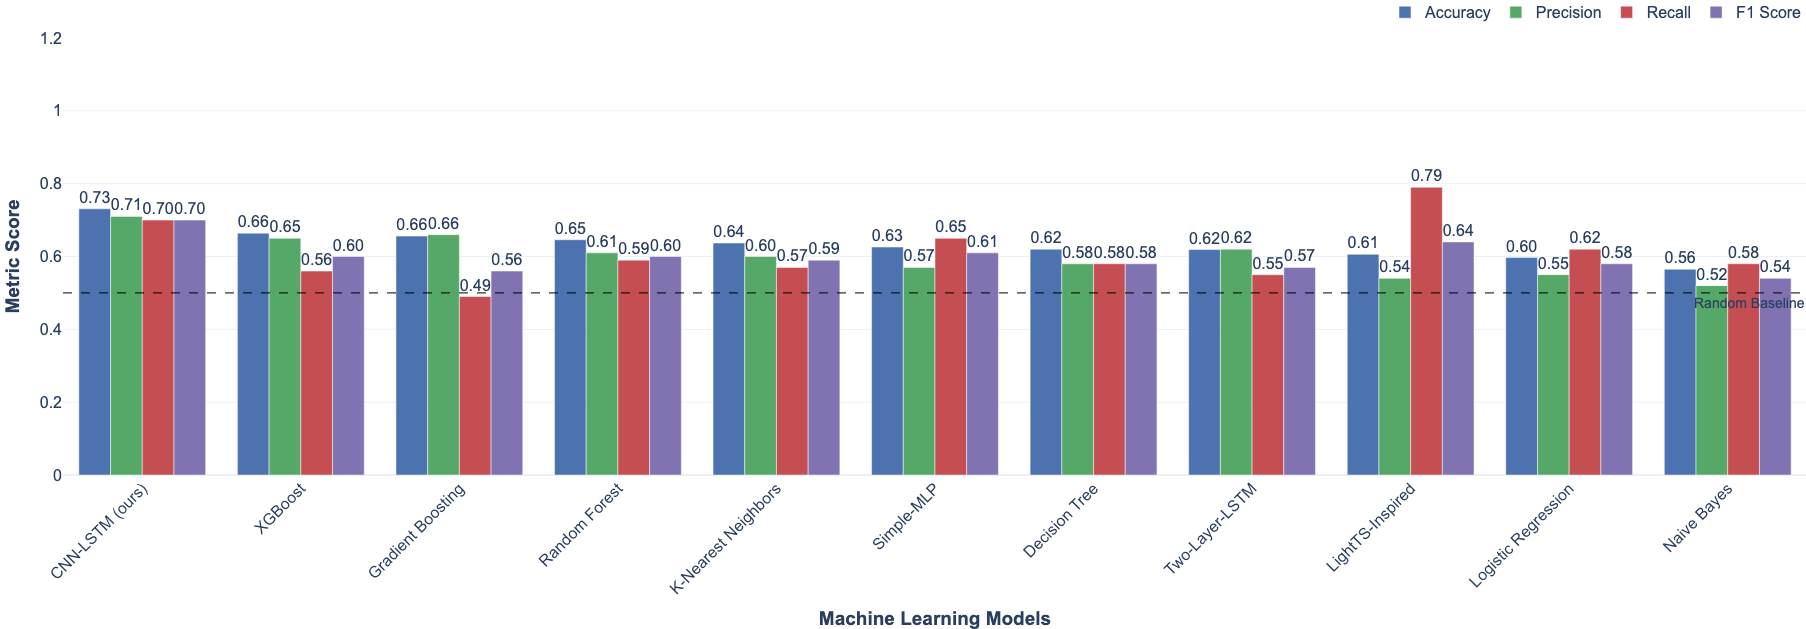
\includegraphics[width=1\textwidth]{images/model_comparision.png}
    \caption{Model Comparison}
    \label{fig:model_comparisons}
\end{figure*}

\begin{figure}[!h]
    \centering
    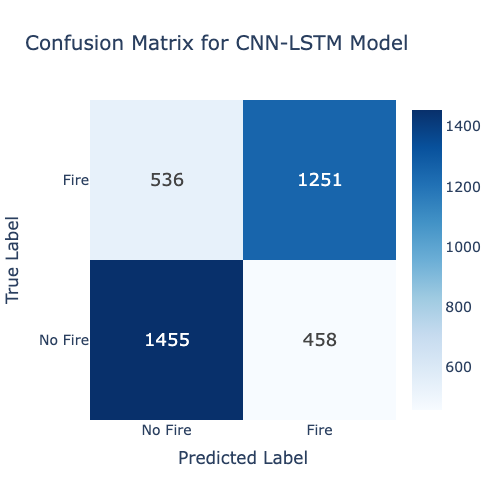
\includegraphics[width=0.75\linewidth]{images/cnn_lstm_confusion_matrix.png}
    \caption{Confusion Matrix}
\end{figure}

\small \textbf{NOTE*} Some portion of the training and testing set are attributed to human causes rather than to natural causes. Since our predictor model primarily relies on weather data, and does not capture data related to human intervention - it can not detect some historical human-caused wildfires. The overall classification metrics of our predictor model reflect this and thus some samples remain unexplained by the model. This limitation highlights the need to add a human activity dimension to our dataset for a more comprehensive wildfire prediction.
\subsection{Helitack Suppression Performance}

\paragraph{Training Performance.} After $3{\times}10^{5}$ training steps, our PPO-based helitack agent reliably learned a circling behavior around the flame front, effectively slowing fire progression in held-out simulation maps.

% After $3{\times}10^{5}$ training steps, the agent with the custom PPO Helitack policy reliably "circles" the flame front and slows growth in held-out terrains.

\subsubsection{Training Setup}

\paragraph{Parallelized Environments.} To promote policy generalization, we trained across 8 real-world wildfire environments (Table~\ref{tab:wildfire_envs_details}) using \texttt{SubprocVecEnv} for simulation parallelism. We applied \texttt{VecNormalize} to stabilize observation scales and improve convergence.

% \paragraph{Vectorized Environment and Normalization}
% To improve training efficiency and policy generalization, we exposed our agent to a variety of scenarios with different environment configurations ie. different land-cover maps and elevations. 
% We used Subprocess Vectorization(\texttt{SubprocVecEnv}) to enable parallel simulations across 8 different environments from 8 real world Wildfires from the history of the United States as shown in Table~\ref{tab:wildfire_envs_details}.

\begin{table}[h!]
\centering
\caption{Wildfire simulation environments used for training, with corresponding fire name, location and dates}
\label{tab:wildfire_envs_details}
\renewcommand{\arraystretch}{1.2}
% \begin{tabular}{|c|l|l|l|}
\begin{tabular}{|c|p{2.5cm}|p{3cm}|p{1.5cm}|}
\hline
\textbf{\#} & \textbf{Fire Name} & \textbf{Location} & \textbf{Date(s)} \\
\hline
1 & Palisades Fires & Los Angeles County, CA & 07 Jan 2025\\
\hline
2 & Lightning Siege & Angeles National Forest, CA & 15 Aug 2020\\
\hline
3 & August Complex Fire & California, USA & 16 Aug 2020\\
\hline
4 & Smokehouse Creek Fire & Texas / Oklahoma, USA & 26 Feb 2024\\
\hline
5 & Yellowstone Fires & WY / MT / ID, USA & 23 Jun 1988\\
\hline
6 & Carlton Complex Fire & Washington, USA & 14 Jul 2014\\
\hline
7 & Okanogan Complex Fire & Washington, USA & 15 Aug 2015\\
\hline
8 & Biscuit Fire & OR / CA, USA & 12 Jul 2002\\
\hline
\end{tabular}
\label{tab:wildfire-envs}
\end{table}

% This parallelism accelerates data collection for PPO updates and helps expose the agent to diverse fire dynamics within each batch. Additionally, we applied observation normalization using \texttt{VecNormalize} to stabilize learning by ensuring consistent feature scaling across episodes. Together, these techniques contributed to faster convergence and improved policy generalization.

\paragraph{HPC Deployment.}
Since our environment combines a Python-based Gymnasium interface with a browser-based fire engine controlled via WebSocket, training is both CPU and GPU intensive. To overcome this, we adopted a headless training strategy using Pyppeteer \cite{pyppeteer} which allows JavaScript code execution without rendering a graphical browser interface.

The entire training setup was containerized into 3 separate containers using Apptainer\cite{apptainer}:
\begin{enumerate}
    \item A Python-based Gymnasium environment with the WebSocket server.
    \item A React + Three.js application for rendering and fire dynamics computation.
    \item A Pyppeteer module for running browser-side code in headless mode.
\end{enumerate}

We trained the model on CCR's high-performance computing cluster \cite{ccr} using custom callbacks for memory cleanup, learning rate scheduling, and checkpointing.

% We use several callbacks to assist in the training:
% RewardLoggingCallback - To log rewards at each step, LearningRateScheduleCallback - A simple LR scheduler to reach maxima, MemoryCleanupCallback - To cleanup memory for resource optimization during training, EpisodePauseCallback - A fallback to save the PPO agent if the training is interrupted(The agent is trained in multiple iterations.)

\subsubsection{Helitack Agent Evaluation}

We compared the trained agent against a rule-based agent. The rule-based agent is a simple helitack agent that tries to extinguish the fire following a simple rule. The agent navigates around the fire in concentric circles, dropping helitacks without using the observation space of the burning fire.

\begin{table*}[htbp]
\centering
\caption{Comparison between Trained PPO Agent and Rule-Based Agent}
\begin{tabular}{|l|c|c|}
\hline
\textbf{Metric} & \textbf{Trained PPO Agent} & \textbf{Rule-Based Agent} \\
\hline
Simulation Screenshot & 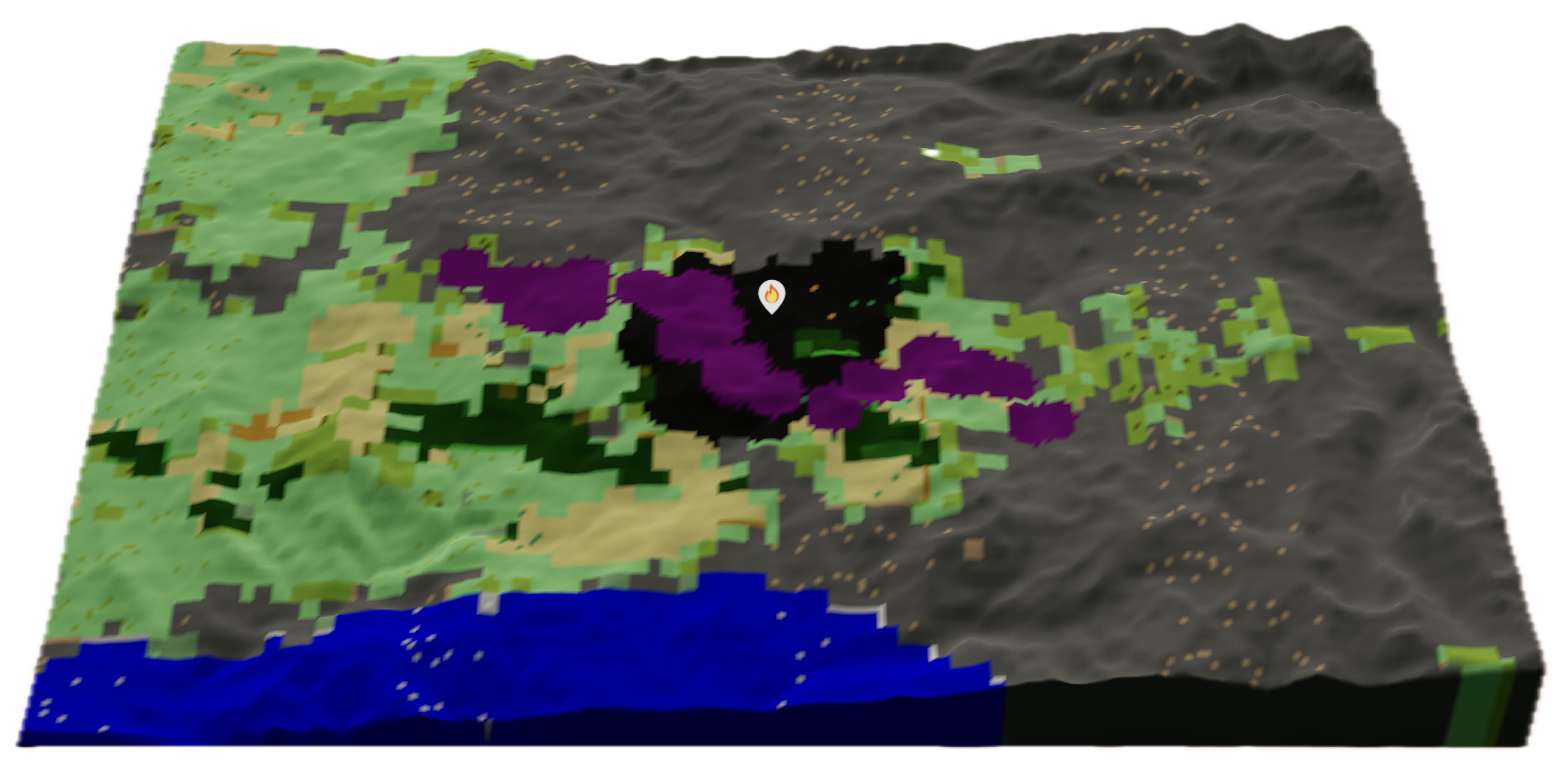
\includegraphics[width=0.3\textwidth]{images/trained_agent_sim.png} & 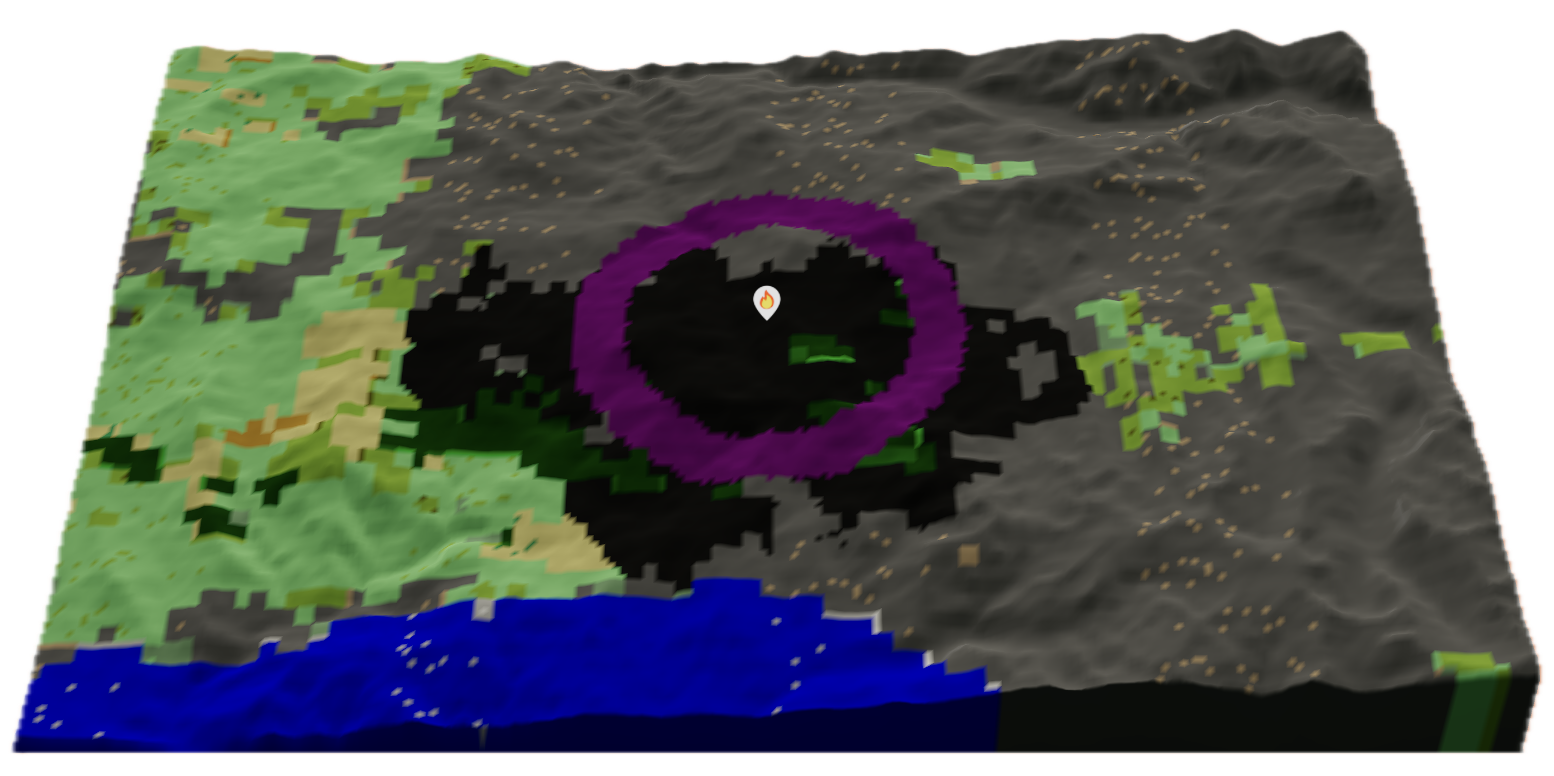
\includegraphics[width=0.3\textwidth]{images/rule_based_agent_sim.png} \\
\hline
Cells burned in episode & 1529 & 4931 \\
\hline
Timesteps & 410 & 883 \\
% \hline
% Description & Trained agent learns to minimize fire spread & Agent moves in a fixed circle (radius 30 cells) around origin \\
\hline
\end{tabular}
\label{tab:agent_comparison}
\end{table*}

These results demonstrate that pairing a 73.1\% accurate forecaster with a simulation-guided RL agent yields actionable suppression strategies and materially reduces projected damage, while the released dataset provides a large-scale benchmark for the community.

\section{Web based Application}

Snapshot from our deployed web application is presented in Fig.~\ref{fig:web_app}

\begin{figure}[!h]
    \centering
    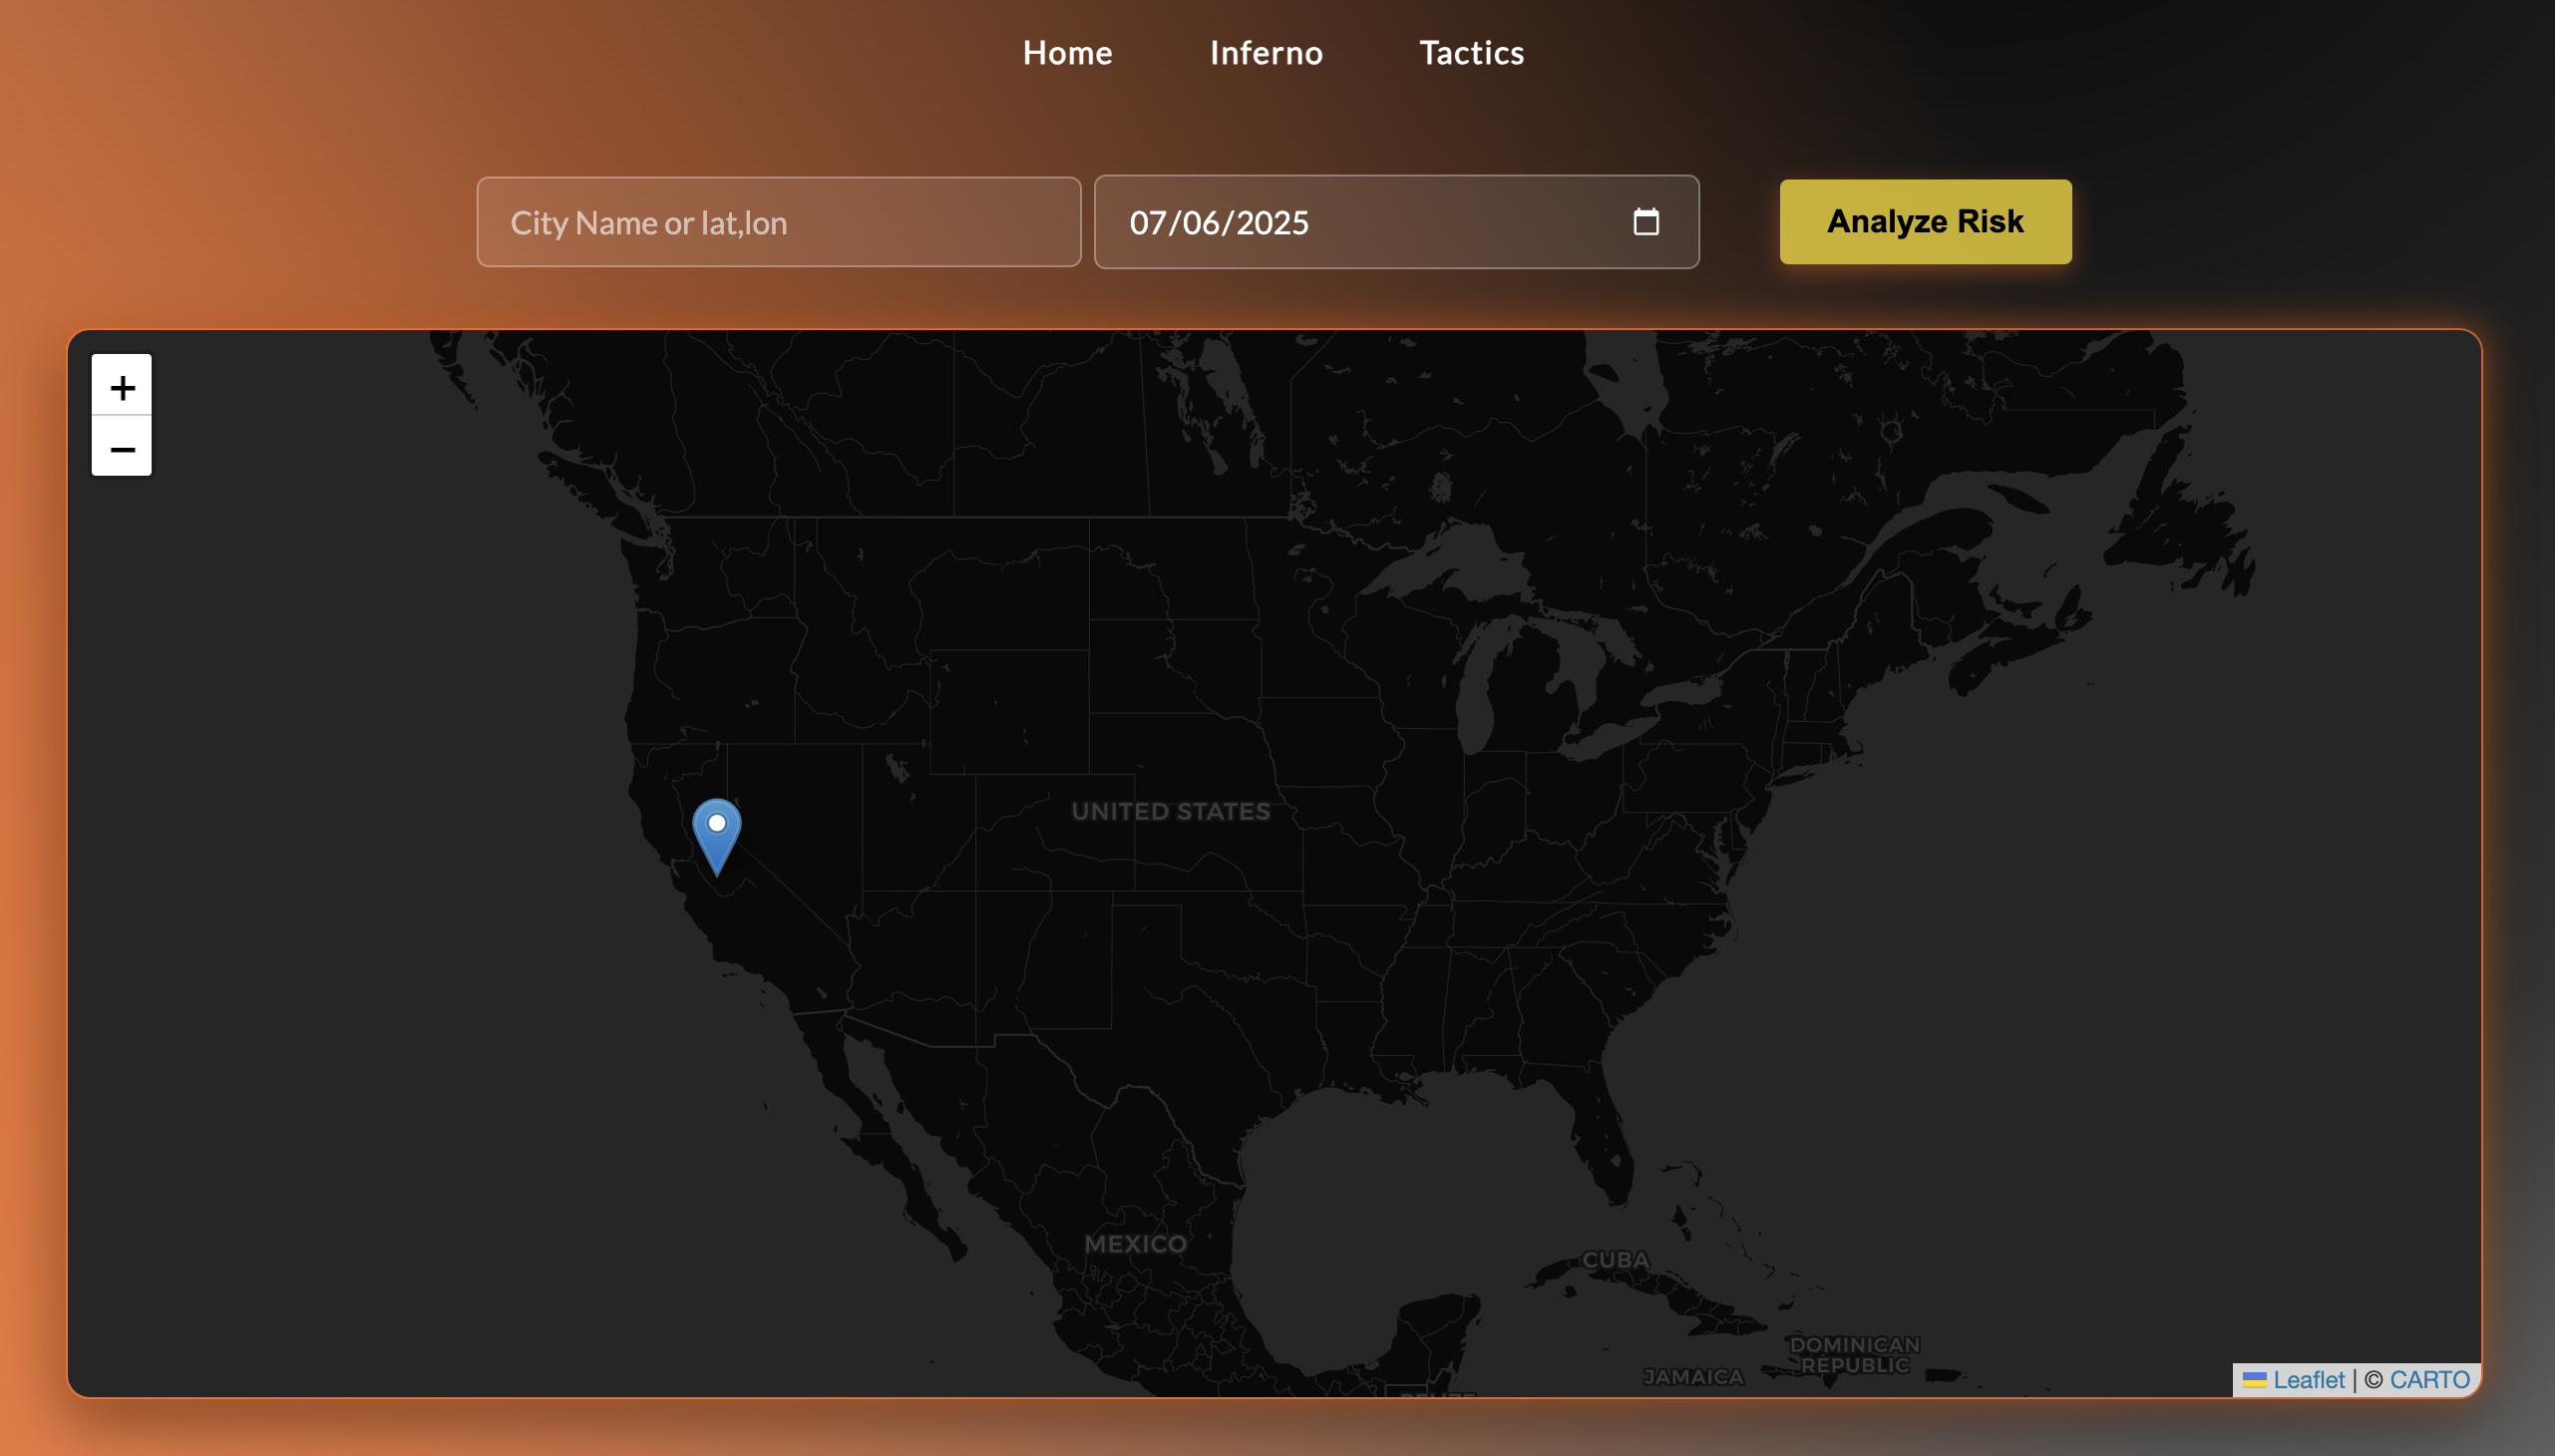
\includegraphics[width=1\linewidth]{images/web_app_inferno.png}
    \caption{Screenshot of the Web Application}
    \label{fig:web_app}
\end{figure}

% We developed a web-based application using Flask and React for users to predict wildfire probability at a location/coordinate. The \textbf{Inferno} UI uses Leaflet which is a navigable map with location picker and calls the backend with the coordinates and date time to make a prediction. The backend uses these coordinates and date time and the calls the GRIDMET API and GRIDMET forecast API to prepare the 75 day window with weather data for the trained model to make a prediction.

% \begin{figure}[!h]
%     \centering
%     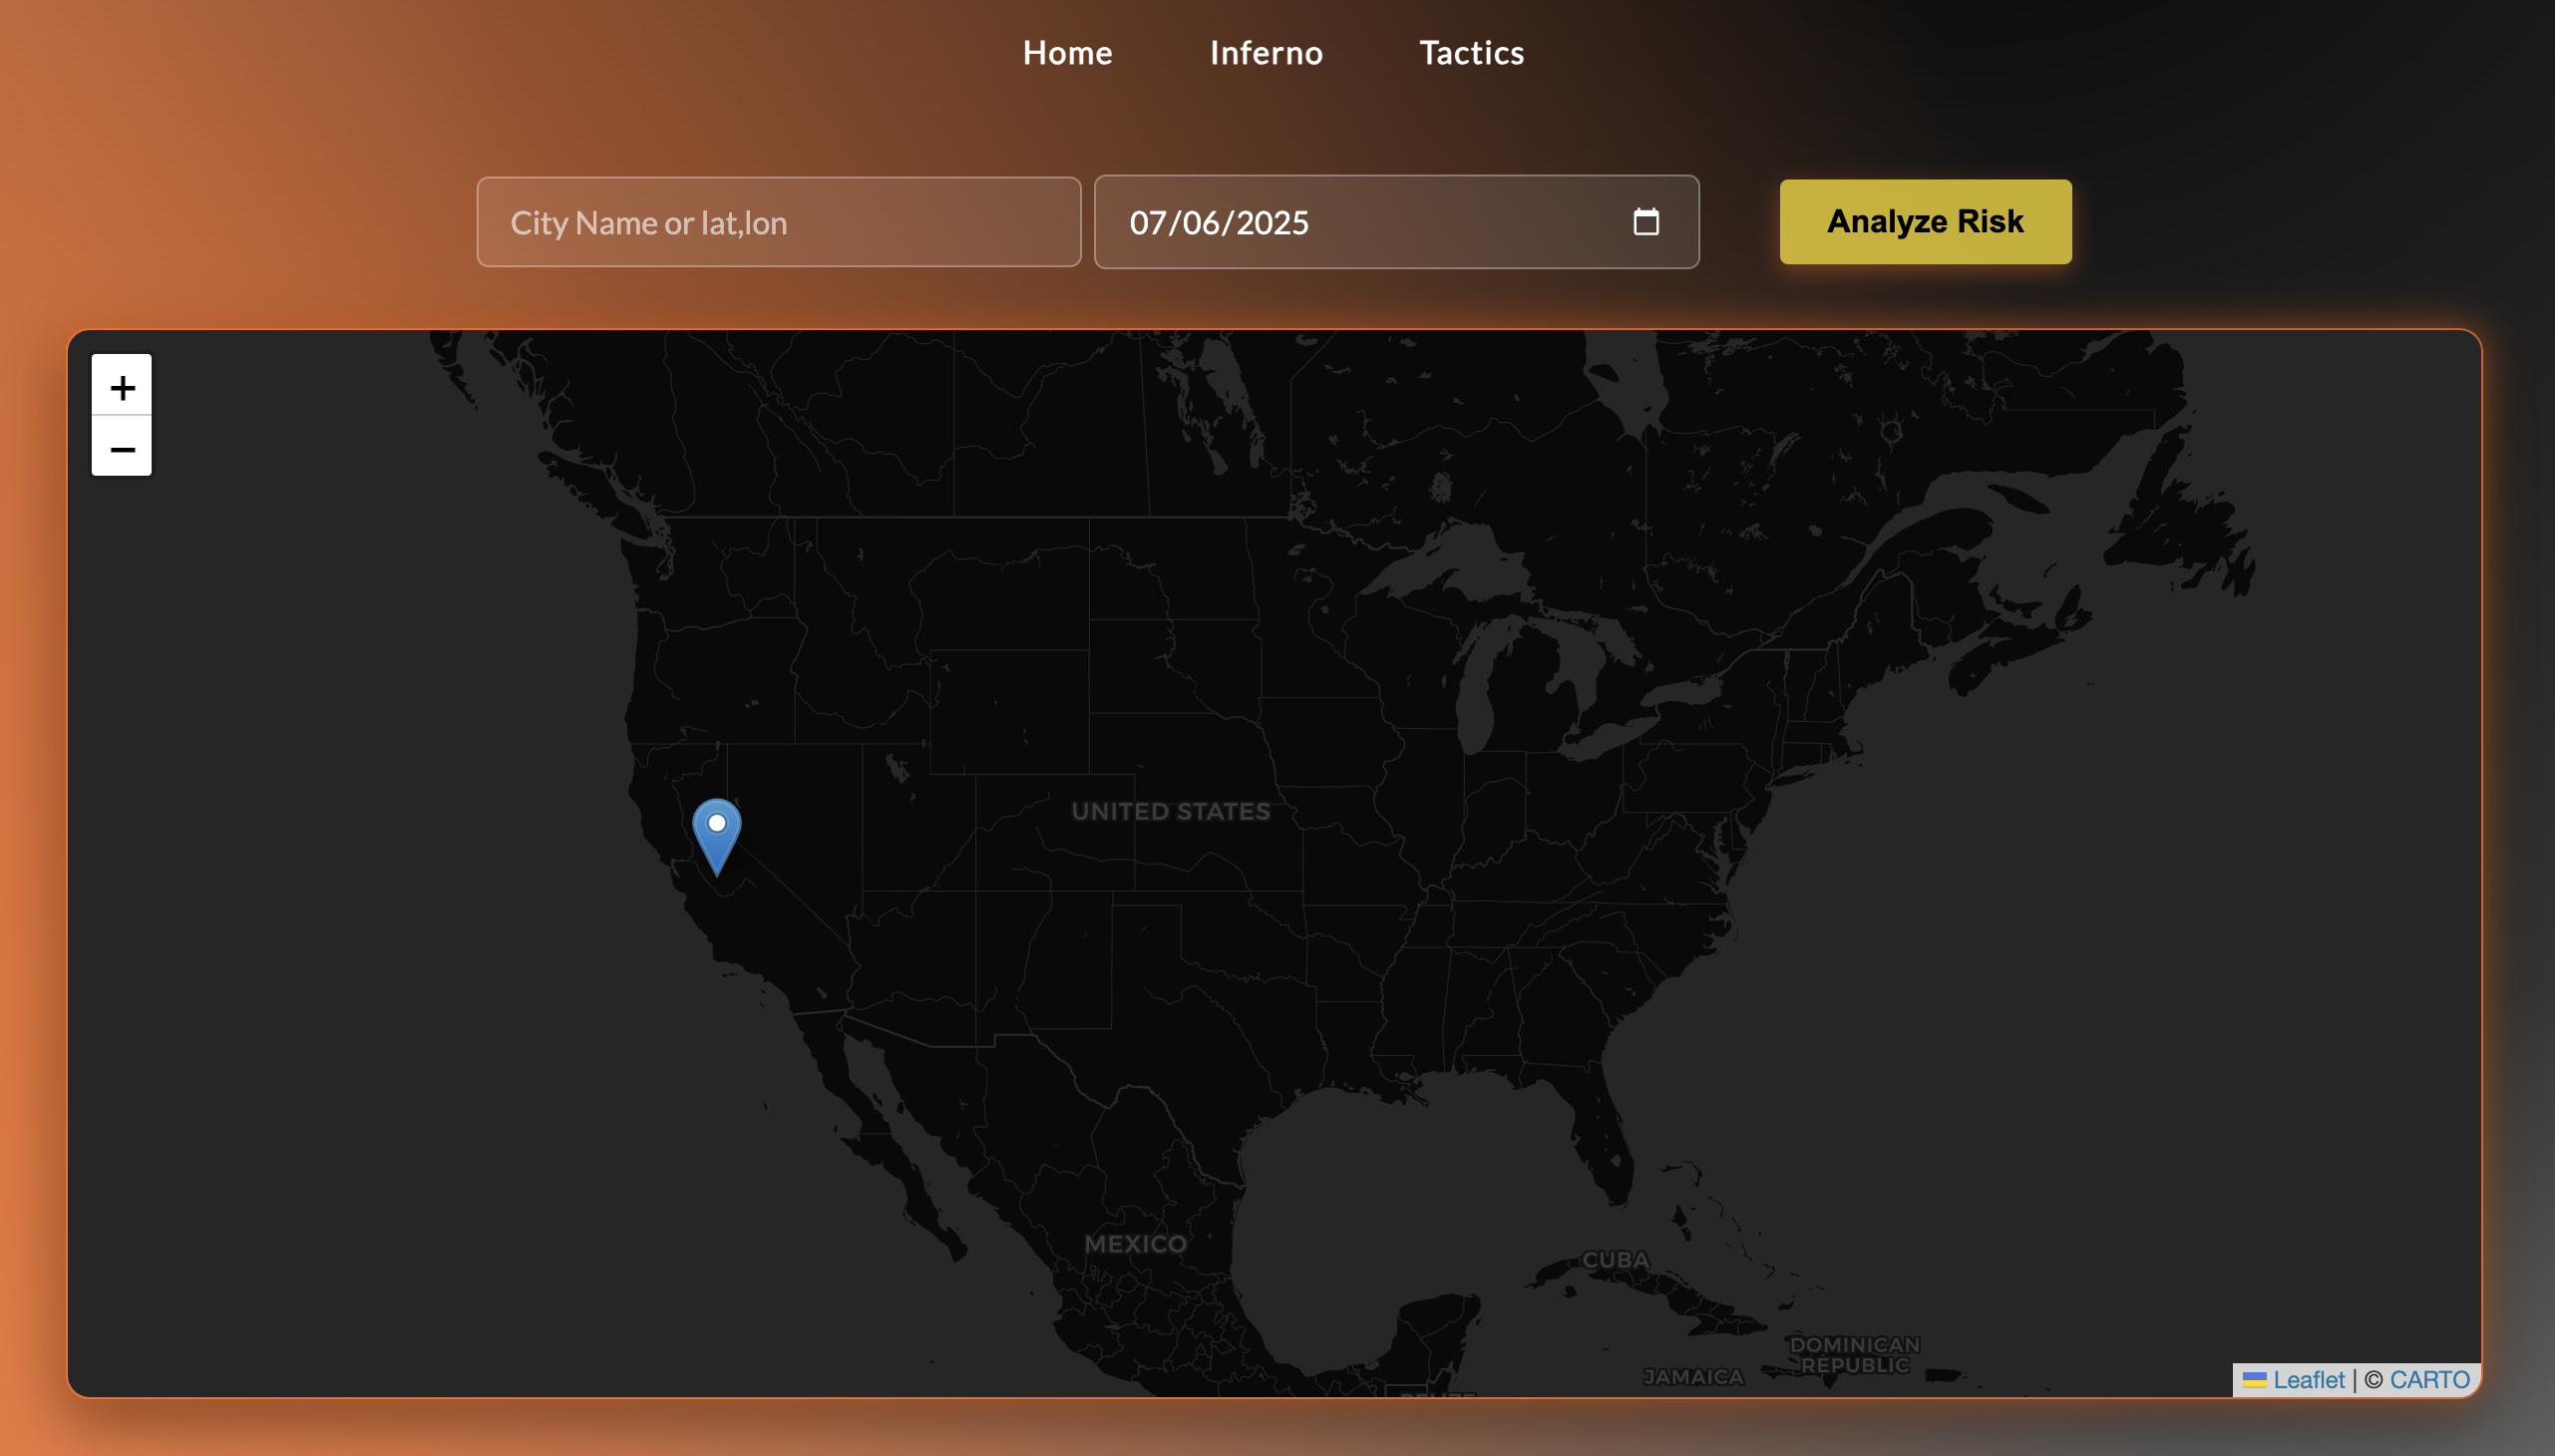
\includegraphics[width=1\linewidth]{images/web_app_inferno.png}
%     \caption{Screenshot of the Web Application}
% \end{figure}

% If the wildfire prediction model predicts a confidence greater than 50\%, we navigate to \textbf{Tactics} (simulation page). The backend then uses the Google Earth Engine python SDK to create the exact cross section of the predicted wildfire using the elevation and land cover data. The trained agent simulates over this rendered environment and tracks the relevant metrics as mentioned in section 4.2 to prepare the Threat assessment report.

\section{Conclusion}
In this work, we introduced an integrated framework that combines deep learning-based wildfire forecasting with reinforcement learning-based suppression tactics in a realistic simulation environment. Beyond the research contributions, this system has strong real-world applicability.

Our RL simulation can be used to develop effective suppression strategies in varied terrains and conditions like \texttt{autonomous fire-fighting drones}. The Threat Assessment Report generated by our pipeline can assist firefighters and policy-makers in planning response by prioritizing high-risk zones and optimizing resource allocation.\\
For example, a team of disaster management responders in a wildfire-prone county can consult our system to assess upcoming wildfire risks and deploy preemptive suppression strategies - effectively turning data into decisive action. This alignment of predictive intelligence with tactical reinforcement learning opens the door to proactive and automated wildfire mitigation.

\section{Suggested Extensions}

We outline several avenues for future enhancement, grouped by pipeline stage.

\subsection{Stage~1 — Forecasting Enhancements}

% \textbf{Incorporate Land‐Cover Layers}: Augment each coordinate–datetime sample with MODIS land‐cover tiles obtained via the Google Earth Engine API to improve spatial context.

% \textbf{Improve metrics \& comparative evaluation}: Benchmark the current CNN–LSTM against other architectures and models (e.g.\ Random Forrest, Gated GRU, Temporal Fusion Transformer, ConvLSTM, ViT) and report richer metrics such as AUROC, PR-AUC, lead-time gain, and false-negative rate.

GAN‐based Consistency Check: Train a conditional generator–discriminator pair in which a novel CNN discriminator judges whether a satellite image truly depicts an ignition event, reinforcing the main classifier and reducing label noise.

Architectural Exploration: Experiment with transformer–CNN hybrids, temporal attention, and cost‐sensitive loss functions to raise overall accuracy and, in particular, drive down false negatives.

\subsection{Stage~2 — Simulation and Control}

% \textbf{Richer Environment State}: Render land‐cover masks and real‐time wind vectors inside the Three.js scene to better align suppression tactics with surface fuels and weather.

% \textbf{Meta Reinforcement Learning}: Generalize the Helitack agent from a single terrain cross‐section to arbitrary topography and fuel types via meta‐learning or domain‐randomisation.

Multi‐Modal Suppression Agents: Introduce additional firefighting primitives—e.g.\ firelines, ground crews, \hbox{CO\textsubscript{$2$}} bombs—and coordinate them through hierarchical or multi‐agent RL.

Open-Source Python–JS Bridge: Refactor the custom Web-socket code that links the Gymnasium environment to the React/Three.js browser renderer into a standalone Python–JavaScript library and release it under an open license to accelerate browser-based RL research.

\subsection{Stage~3 — Reporting and Decision Support}

LLM‐Driven Brief Generation: Replace the current template‐based PDF composer with a large language model that contextualizes simulation logs and assembles stakeholder‐specific prose.

Fire‐Intensity Metrics: Compute per‐pixel fireline intensity and include heat maps to inform resource prioritization.

Actionable Insight Layer: Automatically derive "next-step'' recommendations—e.g.\ staging areas, crew allocations, contingency triggers—tailored to the intensity map and predicted spread.

% \section*{Acknowledgment}

% This research was carried out under the guidance and supervision of \textbf{Prof.\ Alina Vereshchaka}. We thank her for her invaluable advice, critical feedback, and continuous encouragement throughout every stage of this work.

% \begin{thebibliography}{00}
% \bibitem{IRWIN_database} Data Management - Integrated Reporting of Wildfire Information (IRWIN), https://www.wildfire.gov/application/irwin-integrated-reporting-wildfire-information

% \bibitem{gridmet} https://www.climatologylab.org/gridmet.html

% \bibitem{ccr} Center For Computational Research, https://docs.ccr.buffalo.edu/en/latest/

% \bibitem{concord_consortium} Concord Consortium Wildfire Model, https://wildfire.concord.org/

% \bibitem{concord_consortium_github} Concord Consortium Wildfire Model GitHub, https://github.com/concord-consortium/wildfire-model/tree/master/src

% \bibitem{earth_engine} https://developers.google.com/earth-engine/tutorials/community/intro-to-python-api

% \bibitem{ref_article1} Author, F.: Article title. Journal \textbf{2}(5), 99--110 (2016)

% \bibitem{ref_lncs1} Author, F., Author, S.: Title of a proceedings paper. In: Editor, F., Editor, S. (eds.) CONFERENCE 2016, LNCS, vol. 9999, pp. 1--13. Springer, Heidelberg (2016). \doi{10.10007/1234567890}

% \bibitem{ref_book1} Author, F., Author, S., Author, T.: Book title. 2nd edn. Publisher, Location (1999)

% \bibitem{ref_proc1} Author, A.-B.: Contribution title. In: 9th International Proceedings on Proceedings, pp. 1--2. Publisher, Location (2010)

% \bibitem{ref_url1} LNCS Homepage, http://www.springer.com/lncs, last accessed 2023/10/25
% \end{thebibliography}

\bibliographystyle{IEEEtran}
\bibliography{references}


\end{document}
